\documentclass[officiallayout,final]{unihelcompling}
\usepackage[comma, authoryear]{natbib}
\usepackage[all]{xy}
\usepackage{float}
\usepackage{amsmath}
\usepackage{amssymb}
\usepackage{graphicx}
\usepackage{caption}
\usepackage{xltxtra}
%\usepackage{utf8}[inputenc]
\usepackage{xunicode}
\usepackage{subcaption}%,showframe}
\usepackage{setspace}
\usepackage{breqn}
\usepackage{epigraph}
\usepackage{bibentry}
\usepackage{fancyhdr}
\usepackage{fancyvrb}
\usepackage{pdfpages}
%\setcounter{tocdepth}{1}
%\setcounter{chapter}{1}
\captionsetup{compatibility=false}

\usepackage{multirow}
\usepackage[normalem]{ulem}

% Define float-type for algorithms.
\floatstyle{plaintop}
\newfloat{algorithm}{!p}{alg}[chapter]
\floatname{algorithm}{Algorithm}

\usepackage{color}
\usepackage[procnames]{listings}
\usepackage{setspace}

\definecolor{keywords}{RGB}{0,155,155}
\definecolor{comments}{RGB}{155,0,0}
\definecolor{string}{RGB}{0,155,0}
\definecolor{green}{RGB}{0,155,0}
\definecolor{lblue}{RGB}{240,240,255}

\lstset{language=Python, 
        backgroundcolor=\color{lblue},
        basicstyle=\ttfamily\footnotesize, 
        keywordstyle=\color{keywords},
        commentstyle=\color{comments},
        stringstyle=\color{string},
        showstringspaces=false,
        identifierstyle=\color{green},
        numbers=left,
        procnamekeys={def,class,continue,break,if,else,for, return}}
\lstset{escapeinside={(*@}{@*)}}

\renewcommand{\bibsection}{\chapter*{\refname}}

\setmainfont[Mapping=tex-text]{Liberation Serif}

\def\ci{\perp\!\!\!\perp}

\renewcommand{\P}{\mbox{${\rm P}$}}
\newcommand{\R}{\mbox{$\mathbb R$}}
\newcommand{\cond}{\mbox{$ \, | \, $}}
\newcommand{\parcond}{\mbox{$ ; \, $}}
\newcommand{\fw}{\mbox{${\rm fw}$}}
\newcommand{\bw}{\mbox{${\rm bw}$}}
\newcommand{\Z}{\mbox{${\rm Z}$}}
\newcommand{\data}{\mbox{${\mathcal{D}}$}}
\DeclareMathOperator*{\argmax}{arg\,max}
\DeclareMathOperator*{\argmin}{arg\,min}
\renewcommand{\O}{\mbox{${\rm O}$}}
\title{Morphological Disambiguation using \\ Probabilistic Sequence Models}
\author{Miikka Pietari Silfverberg}
\authorcontact{\url{mpsilfve@iki.fi}\par
\url{http://www.iki.fi/\textasciitilde mpsilfve}}
\pubtime{Foo}{2016}
\reportno{0}
\isbnpaperback{XXX-XXX-XX-XXXX-X}
\isbnpdf{XXX-XXX-XX-XXXX-X}
%\issn{0000-0000}
\printhouse{Unigrafia Oy}

\supervisorlist{{Krister Lindén, University of Helsinki, Finland}{\\\hangindent=1em Anssi Yli-Jyrä, University of Helsinki, Finland}}
\preexaminera{Prof. Jan Hajič, Charles University in Prague, Czech Republic}
\preexaminerb{Prof. Joakim Nivre, Uppsala University, Sweden}
\opponent{Prof. Joakim Nivre, Uppsala University, Sweden}
\custos{Prof. Jörg Tiedemann, Univeristy of Helsinki, Finland}
\generalterms{morphological tagger, morphological analyzer, POS tagging, HMM, CRF, perceptron}
\additionalkeywords{morphologically complex languages}
%\crcshort{F.1.1, I.2.7, I.7.1}
%\crclong{
%\item}
\permissionnotice{
 Academic dissertation to be publicly discussed, by due permission of the Faculty of Arts at the University of Helsinki in auditorium XYZ, on the 22th of October, 2016 at 10 o’clock.
}
\date{\today}

\begin{document}
\bibstyle{apa}


% Make arrays a bit spacier.
\def\arraystretch{1.2}

\clearpage
%\begin{titlepage}
\begin{center}
Department of Modern Languages\\
2015\\
\vspace*{\fill}
\textsc{\LARGE Morphological Disambiguation using}\\[0.5cm]
\textsc{\LARGE Probabilistic Sequence Models}\\
%(Maybe limit title further)\\
\vspace*{\fill}
\textsc{\large Miikka Pietari Silfverberg}\\
\vspace*{\fill}
\end{center}
{\it Academic dissertation to be publicly discussed, by due permission of
the Faculty of Arts at the University of Helsinki in
LOCATION, on the XXth of Month, 2015 at 12 o{’}clock.}\\
\vspace*{\fill}
\begin{center}
University of Helsinki\\
Finland
\end{center}
\end{titlepage}

\frontmatter
\maketitle
\vspace*{\fill}
\thispagestyle{empty} 
\begin{quotation}
\em % optional -- to switch to emphasis (italics) mode
Nobody is going to read your PhD thesis

\medskip
\raggedleft
Ancient Proverb
\end{quotation}
\vspace*{\fill}
\onehalfspacing

\pagenumbering{roman}
%\begin{abstract}
  A morphological tagger is a piece of computer software that provides
  complete morphological descriptions of sentences. Morphological
  taggers find applications in many NLP fields. For example, they can
  be used as a pre-processing step for syntactic parsers, in
  information retrieval and machine translation. The task of
  morphological tagging is closely related to POS tagging but
  morphological taggers provide more fine-grained morphological
  information than POS taggers. Therefore, they are often applied to
  morphologically complex languages, which extensively utilize
  inflection, derivation and compounding for encoding structural and
  semantic information. This thesis presents work on data-driven
  morphological tagging for Finnish and other morphologically complex
  languages.

  Previous work on data-driven morphological tagging for Finnish is
  scarce because of the lack of freely available manually prepared
  morphologically tagged corpora. The work presented in this thesis is
  made possible by the recently published Finnish dependency treebanks
  FinnTreeBank and Turku Dependency Treebank. Additionally, the
  Finnish open-source morphological analyzer OMorFi is extensively
  utilized in the experiments presented in the thesis.

  The thesis presents methods for improving tagging accuracy,
  estimation speed and tagging speed in presence of large structured
  morphological label sets that are typical for morphologically
  complex languages. More specifically, it presents a novel
  formulation of generative morphological taggers using weighted
  finite-state machines and applies finite-state taggers to context
  sensitive spelling correction of Finnish. The thesis also explores
  discriminative morphological tagging. It presents structured
  sub-label dependencies that can be used for improving tagging
  accuracy. Additionally, the thesis presents a cascaded variant of the
  averaged perceptron tagger. In presence of large label sets, a
  cascaded design results in substantial reduction of estimation speed
  compared to a standard perceptron tagger. Moreover, the thesis
  explores pruning strategies for perceptron taggers. Finally, the
  thesis presents the FinnPos toolkit for morphological
  tagging. FinnPos is an open-source state-of-the-art averaged
  perceptron tagger implemented by the author.
\end{abstract}

\pagenumbering{arabic}

\mainmatter

\tableofcontents
\listoffigures
\listoftables
\listof{algorithm}{List of Algorithms}
\addcontentsline{toc}{chapter}{List of Algorithms}

\chapter*{Notation}
\addcontentsline{toc}{chapter}{Notation}
\begin{tabular*}{\columnwidth}{@{\extracolsep{\stretch{1}}}*{2}{l}@{}}
\multicolumn{2}{c}{Acronyms}\\
CRF  & Conditional Random Field                          \\
HMM  & Hidden Markov Model                               \\
MEMM & Maximum-Entropy Markov Model                      \\
NB   & Na\"{i}ve Bayes                                   \\
PGM  & Probabilistic Graphical Model                     \\
POS  & Part-of-Speech                                    \\
MAP  & Maximum a posteriori                              \\
     & \\
\multicolumn{2}{c}{Mathematical Notation}\\
$x[1:t]$ & Prefix $(x_1,\ ...,\ x_t)$ of sequence $x = (x_1,\ ...,\ x_t,\ ...,\ x_T)$.\\
$X^t$    & The cartesian product of $t$ copies of the set $X$.
\end{tabular*}

\chapter*{Acknowledgements}
\addcontentsline{toc}{chapter}{Acknowledgements}
%Teemu Ruokolainen statistical methods, friendship, writing.
%
%Måns Huld\'{e}n finite-state, statistical methods, inspiration,
%courage, IPA.
%
%Krister Lind\'{e}n ideas, letting me do useless stuff once in a while,
%pushing me forward, encouragement, realism.
%
%Anssi Yli-Jyrä inspiration, finite-state, positive attitude, friendship.
%
%Kimmo Koskenniemi intellectual rigorosity, how to think of stuff, how
%to be legible, being critical.
%
%Arto Voutilainen
%
%Erik Axelson
%
%Tommi Pirinen
%
%Senka Drobac
%
%Sam Hardwick
%
%Graham Wilcock 
%
%Juliette Kennedy
%
%Panu Kalliokoski
%
%Coursera
%
%Reetta Vuokko-Syrjänen and Kaj Syrjänen + Elsa
%
%Family
%
%Veera Nykänen
%
%Jarmo Widemann
%
%Antti, Sami, Ville, Jarmo, Rod, Marko and many more friends who have
%brought a lot of happiness through the time I've been working on this
%thesis project.
%

\chapter{Introduction}
\label{ch:intro}

A morphological tagger is a piece of computer software that provides
complete morphological descriptions of sentences. An example is given
in Figure \ref{fig:mt-example}. Each of the words in the sentence is
assigned a detailed morphological label, which specifies
part-of-speech and inflectional information. Each word also receives a
lemma. Morphological tagging is typically a pre-processing step for
other language processing applications, for example syntactic parsers,
machine translation software and named entity recognizers.

The task of morphological tagging is closely related to part-of-speech
tagging (POS tagging), where the words in a sentence are tagged using
coarse morphological labels such as noun and verb. These typically
correspond to main word classes. POS taggers are sufficient for
processing languages where the scope of productive morphology is
restricted, for example English. Morphological taggers are, however,
necessary when processing {\it morphologically complex languages}, which
extensively utilize inflection, derivation and compounding for
encoding structural and semantic information. For these languages, a
coarse POS tag simply does not provide enough information to enable
accurate downstream processing such as syntactic parsing.\footnote{For
  example in Finnish, the subject and object of a sentence are
  distinguished by case and different verbs can require different
  cases for their arguments \cite{Hakulinen2004}. Coarse POS tags do
  not capture such distinctions. Therefore, accurate parsing of
  Finnish cannot rely solely on coarse POS tags.}

\begin{figure}[!htb]
\begin{center}
\begin{tabular}{|l|l|l|l|l|l|l|}
\hline
Article+Indef & Noun+Sg & Verb+Pres+3sg & Prep & Article+Def & Noun+Sg & .\\  
\hline
\textsc{a} & dog & sleep & on & the & mat & .\\
\hline
A & dog & sleeps & on & the & mat & .\\
\hline
\end{tabular}
\end{center}
\caption{A morphologically tagged sentence}\label{fig:mt-example}
\end{figure}

At first glance, the task of assigning morphological descriptions, or
{\it morphological labels}, seems almost trivial. Simply form a list of
common word forms and their morphological labels and look up words in
the list when tagging text. Unfortunately, this approach
fails because of the following reasons.

\begin{enumerate}
\item A single word form can get several morphological labels
  depending on context. For example ``dog'' and ``man'' can be both
  nouns and verbs in English.
\item For morphologically complex languages, it is impossible to form a
  list of common word forms which would have sufficient coverage (say,
  higher than 95\%) on unseen text.
\end{enumerate}

Due to the reasons mentioned above, a highly accurate morphological
tagger must model the context of words in order to be able to
disambiguate between their alternative analyses. Moreover, it has to
model the internal structure of words in order to be able to assign
morphological labels for previously unseen word forms based on similar
known words.

This thesis presents work on building morphological taggers for
morphologically complex languages, in particular Finnish, which is the
native language of the author. The thesis focuses on data-driven
methods which utilize manually prepared training corpora and machine
learning techniques for learning tagger models.

\section{Motivation}
Data-driven methods have dominated the field of natural language
processing (NLP) since the 1990's. Although these methods have been
applied to virtually all language processing tasks, research has
predominantly focused on a few languages, English in particular. For
many languages with fewer speakers, such as Finnish, statistical
methods have not been applied to the same extent. This is probably due
to the fact that large training corpora required by supervised
data-driven methods are available for very few languages.

The relative lack of work on statistical NLP for languages besides English is a
problem because the languages of the world differ substantially with
regard to syntax, morphology, phonology and orthography. These
differences have very real consequences for the design of NLP
systems. Therefore, it is impossible to make general claims about
language processing without testing the claims on other languages
in addition to English.

This thesis presents work that focuses on data-driven methods for
morphological tagging of Finnish. Finnish and English share many
characteristics but also differ in many respects. Both are written in
Latin script using similar character inventories, although Finnish
orthography uses three characters usually not found in English text
``å'', ``ä'' and ``ö''. Moreover, there are similarities in the
lexical inventories of the languages because, like many modern
languages, Finnish has been influenced by English and because both
languages are historically associated with Germanic and Nordic
languages. In some respects, however, Finnish and English are vastly
different. Whereas English has fixed SVO word order, the word order in
Finnish is quite flexible. Another major difference is the amount of
inflectional morphology. For example, English nouns usually only occur
in three inflected forms: singular ``cat'', plural ``cats'' and
possessed ``cat's''. In contrast, thousands of inflected forms can be
coined from a single Finnish noun.

Although data driven methods have dominated the field of POS tagging
and, to a lesser extent, morphological tagging for the last twenty
years, data driven work on Finnish morphological tagging has been
scarce mostly because of the lack of high quality manually annotated
broad coverage training corpora. However, other approaches like the
purely rule based constraint grammar \citep{Karlsson1995} and its
derivative functional dependency grammar \citep{Tapanainen1997} have
been successfully applied for joint morphological tagging and
shallow parsing.\footnote{For example, the Finnish constraint grammar
  tagger FinCG is available online through the GiellaTekno Project
  %\citep{gt}
  \url{https://victorio.uit.no/langtech/trunk/kt/fin/src/fin-dis.cg1}
  (fetched on February 24, 2016).}

The recently published FinnTreeBank \citep{Voutilainen2011} and Turku
Dependence Treebank \citep{Haverinen2013} represent the first freely
available broad coverage Finnish hand labeled data sets that can be
used for work on morphological tagging. These resources enable
experiments on statistical morphological tagging for Finnish using a
convincing gold standard corpus. Moreover, the broad coverage
open-source Finnish morphological analyzer OMorFi \citep{Pirinen2011}
is a valuable resource for improving the performance of a tagging
system.

The complex morphology present in the Finnish language leads to problems
when existing tagging algorithms are used. The shear amount of
possible morphological analyses for a word slows down both model
estimation and application of the tagger on input text. Moreover, the
large amount of possible analyses causes data sparsity
problems. %Another problem is caused by productive compounding and
%extensive inflection.  

Data driven methods typically perform much
worse on so called out-of-vocabulary (OOV) words, that is words which
are missing from the training corpus, than on words seen during
training. In English, this is usually not detrimental to the
performance of the tagger, because the amount of OOV words is
typically rather low. In contrast, this becomes a substantial problem
for purely data driven systems processing morphologically complex
languages because productive compounding and extensive inflection lead
to a large amount of OOV words even within the same domain.

%\begin{itemize}
%\item Data-driven methods have been very successful in dealing with
%  English language technology.
%\item Morphologically complex language present problems for many statistical approaches.
%\item Data sparsity because of large vocabularies.
%\item Data sparsity because of large label sets.
%\item Model estimation is slow.
%\item Data sets are typically small.
%\item Most work on Finnish morphological tagging and disambiguation
%  has centered on purely expert driven systems such as Constraint
%  grammar.
%\item Wanted to investigate statistical methods.
%\item OMorFi, the open morphological analyzer and FTB and TDT allow
%  for work on statistical tagging of Finnish..
%\end{itemize}

\section{Main Contributions}

This thesis presents an investigation into data-driven morphological
tagging of Finnish both using generative and discriminative
models. The aim of my work has been creation of practicable taggers
for morphologically complex languages. Therefore, the main contributions
of this thesis are practical in nature. I present methods for
improving tagging accuracy, estimation speed, tagging speed and reducing
model size. More specifically, the main contributions of the thesis
are as follows.

\begin{itemize}
\item {\bf A novel formulation of generative morphological taggers
    using weighted finite-state machines} Finite-state calculus allows
  for flexible model specification while still guaranteeing efficient
  application of the taggers. Traditional generative taggers, which
  are based on the Hidden Markov Model (HMM), employ a very limited
  feature set and changes to this feature set require modifications to
  the core algorithms of the taggers. Using weighted finite-state
  machines, a more flexible feature set can, however, be employed
  without any changes to the core algorithms. This work is presented
  in Publications \ref{pub:1} and \ref{pub:2}.
\item {\bf Morphological taggers and POS taggers are applied to context
  sensitive spelling correction} Typically, context sensitive spelling
  correctors rely on neighboring words when estimating the probability
  of correction candidates. For morphologically complex languages, this
  approach fails because of data sparsity. Instead, a generative
  morphological tagger can be used score suggestions based on
  morphological context as shown in Publication \ref{pub:3}.
\item {\bf Feature extraction specifically aimed at morphologically
    complex languages} As mentioned above, the large inventory of
  morphological labels causes data sparsity problems for morphological
  tagging models such as the averaged perceptron and conditional
  random field. Using sub-label dependencies presented in Publication \ref{pub:5},
  data sparsity can, however, be alleviated. Moreover, sub-label
  dependencies allow for modeling congruence and other similar
  syntactic phenomena.
\item {\bf Faster estimation for perceptron taggers} Exact estimation
  and inference is infeasible in discriminative taggers for
  morphologically complex languages because the time requirement of exact
  estimation and inference algorithms depends on the size of the
  morphological label inventory which can be quite large. Some design
  choices (like higher model order) can even be impossible for
  morphologically complex languages using standard tagging
  techniques. Although the speed of tagging systems is not always seen
  as a major concern, %I believe that both estimation and tagging speed
  %is important. 
  it can be important in practice.
A faster and less accurate tagger can often be
  preferable compared to more accurate but slower taggers in real world
  applications where high throughput is vital. Estimation speed, in
  turn, is important because it affects the development process of the
  tagger. For these reasons, Publications \ref{pub:4} and \ref{pub:5}
  explore known and novel approximate inference and estimation
  techniques. It is shown that these lead to substantial reduction in
  training time and faster tagging time compared to available
  state-of-the-art tagging toolkits.
\item {\bf Pruning strategies for perceptron taggers} Model size can
  be a factor in some applications. For example, when using a tagger
  on a mobile device. In Chapter \ref{chapter:crf}, I review different
  techniques for feature pruning for perceptron taggers and present
  some experiments on feature pruning in Chapter
  \ref{chapter:finnpos}.
\item {\bf FinnPos toolkit.} Publication \ref{pub:6} presents FinnPos,
  an efficient open source morphological tagging toolkit for Finnish
  and other morphologically complex languages. Chapter
  \ref{chapter:finnpos} presents a number of experiments on
  morphological tagging of Finnish using the FTB and TDT
  corpora. These experiments augment the results presented in
  Publication \ref{pub:6}.
\end{itemize}

%\begin{itemize}
%\item Investigation of statistical morphological tagging for Finnish.
%\item A formulation of generative taggers using finite-state machines
%  which allows for generalizations of the usual HMM tagger
%  formulation.
%\item Investigation of using a POS tagger to improve spelling
%  correction. Comparison against word n-grams show that POS tags
%  perform better.
%\item A new way to specify structued features.
%\item Faster estimation compared to other state-of-the-art toolkits.
%\item Investigation into averaged perceptron model pruning.
%\item FinnPos toolkit.
%\end{itemize}

\section{Outline}
This thesis can be seen as an introduction to the field of
morphological tagging and the techniques used in the field. It should
give sufficient background information for reading the articles that
accompany the thesis. Additionally, Chapter \ref{chapter:finnpos} of
the thesis presents detailed experiments using the FinnPos
morphological tagger that were not included in Publication
\ref{pub:6}.

Chapter \ref{chap:morphology} establishes the terminology on
morphology and morphological tagging as well as surveys the field of
morphological tagging.  Chapter \ref{chap:ml} is a brief introduction
to supervised machine learning and the experimental methodology of
natural language processing.  In Chapter \ref{chapter:hmm}, I
introduce generative data-driven models for morphological tagging.
Chapter \ref{chap:fsm} introduces finite-state machines and a
formulation of generative morphological taggers in finite-state
algebra. It also shows how finite-state algebra can be used to
formulate generative taggers in a generalized manner encompassing
both traditional HMM taggers and other kinds of models.  Chapter
\ref{chapter:crf} deals with discriminative morphological taggers and
introduces contributions to the field of
discriminative morphological tagging.  Chapter
\ref{chapter:lemmatization} deals with the topic of data-driven
lemmatization. Experiments on morphological tagging using the FinnPos
toolkit are presented in Chapter \ref{chapter:finnpos}. Finally, the
thesis is concluded in Chapter \ref{chapter:conclusions}.


\chapter{Morphology}

\section{The Structure of Words}
\begin{itemize}
\item The morphological system.
\item Word, morpheme, lemma, stem.
\item Word classes.
\item Inflectional categories.
\end{itemize}
\section{Languages with Rich Morphology}
\begin{itemize}
\item Typological classification of languages.
\item ``Large label sets''.
\end{itemize}

\section{Morphological Analyzers}
\begin{itemize}
\item Finite-state morphology \citep{Koskenniemi1984}, \citep{Kaplan1994}.
\end{itemize}

\chapter{Machine Learning}
\label{chap:ml}

This section outlines the basic methodology followed in machine
learning research for NLP. I will briefly
discuss machine learning from a general point of view and then present
supervised machine learning in more detail using linear regression as
example.

\paragraph{Supervised and Unsupervised ML} There exists a broad
division of the field of machine learning into three sub-fields.\footnote{However, for example reinforcement learning and active learning may not fit easily into this classification.}
\begin{enumerate}
\item In {\it supervised} machine learning the aim is to learn a mapping
  from inputs $x$ (such as sentences) to outputs $y$ (such as
  morphological label sequences). To this aim, a supervised system
  uses training material consisting of input-output pairs $(x,y)$ and
  a model which can represent the mapping $x \mapsto y$. Training of
  the model consists of tuning its parameters in such a way that the
  model accurately describes mapping between the inputs and outputs in
  the training data. Typically, supervised machine learning is
  employed for tasks such as classification and regression. Examples
  in the field of natural language processing include POS tagging and
  other tasks that can be framed as labeling (for example named entity
  recognition), speech recognition and machine translation.
\item In contrast to supervised machine translation, {\it unsupervised}
  approaches exclusively utilize unannotated data, that is the
  training data consists solely of inputs $x$. Unsupervised machine
  learning is most often used for various kinds of clustering tasks
  where inputs are grouped into sets of similar examples. Therefore,
  it has applications for example in exploratory data analysis.
\item Finally, {\it semi-supervised}
  systems use an annotated training set in combination with a,
  typically, very large unannotated training set to improve the
  results beyond the maximum achievable by either approach in
  isolation.
\end{enumerate}

Unsupervised and Semi-supervised techniques have many applications in
the field of tagging. For example, distributional similarity can be
used to improve tagging accuracy for OOV words
\citep{Huang2009a,Ostling2013} and self-training can improve the
accuracy of a tagging system \citep{Spoustova2009,Sogaard2011}.  This
thesis, however, focuses exclusively on supervised learning.

\section{Supervised Learning}
%\begin{itemize}
%\item Example: linear regression.
%\item Estimation from a sample.
%\item Convexity, smoothness.
%\item Regularization.
%\item Methodology: Training, development and test sets. 
%\item Significance testing.
%\end{itemize}

In this section, I will illustrate the key concepts and techniques in
supervised machine learning using the very simple example of {\it
  linear regression}. I will explain the plain linear regression model
and show how it can be fitted using training data. I will then briefly
present {\it ridge regression} which is a {\it regularized} version of
linear regression.

I choose linear regression as example because it is a simple model yet
can be used to illustrate many important concepts in machine
learning. Moreover, the model has several tractable properties such as
smoothness and convexity. Additionally, it can be seen as the simplest
example of a linear classifier which is a category of models
encompassing conditional random fields, the hidden Markov model and
average perceptron classifier presented in later chapters.

\paragraph{Linear Regression} As a simple example, imagine a person
called Jill who is a real estate agent.\footnote{This example is
  inspired by the Machine learning course provided by Coursera and at
  the time taught by Andrew Ng.} She is interested in constructing an
application, for use by prospective clients, which would give rough
estimates for the selling price of a property. Jill knows that a large
number of factors affect housing prices. Still, there are a few very
robust predictors of price that are easy to measure.
She decides to base the model on the following predictors:
\begin{enumerate}
\item The living area.
\item The number of rooms.
\item The number of bathrooms.
\item Size of the yard.
\item Distance of the house from the city center.
\item Age of the house.
\item Elapsed time since the last major renovation.
\end{enumerate}

Jill decides to use the simplest model which seems reasonable. This
model is linear regression which models the dependent
  variable, the house price, as a linear combination of the independent
variables listed above and parameter values in $\R$. The linear
regression model is probably not accurate. It fails in several
regards. For example, increasing age of the house probably reduces the
price up to a point but very old houses can in fact be more expensive
then newly built houses especially if they have been renovated lately.
Although, the linear model is unlikely to be entirely accurate, Jill is
happy with it because the intention is just to give a ball park
estimate of the price for the prospective client.

To formalize the linear regression model, let us call the dependent
variable price $y$ and each of the independent variables living area,
number of rooms and so on $x_i$. Given a vector $x = (x_1\ ...\
x_n\ 1)^\top \in \R^{n+1}$, which combines the independent
variables $x_i$, a bias term $1$, and a parameter vector $\theta \in
\R^{n+1}$ the linear regression model is given by Equation
\ref{eq:linreg}.\footnote{In reality, each of the predictors would probably
  be transformed to give all of them the same average and
  variance. Although this ii not required in theory, it tends to give
  a better model.}

\begin{equation}
y(x\parcond \theta) = x^\top\theta\label{eq:linreg}
\end{equation}

Two questions immediately arise: How to compute the price given
parameters and predictors and how to compute the parameter vector
$\theta$. These questions are common for all supervised learning
problems also when using other models than the linear regression
model.

\paragraph{Inference} The first question concerns {\it inference},
that is finding finding the values of the dependent variable given
values for the independent variables. In the case of linear
regression, the answer to this question is straightforward. To compute
the price, simply perform the inner product in Equation
\ref{eq:linreg}. The question is, however, not entirely settled
because one might also ask for example how close to the actual price
the estimate $y$ is likely to be. A related question would be to
provide an upper and lower bound for the price so that the actual
price is very likely to be inside the provided bounds. To answer these
questions, one would have to model the expected error.

Inference is very easy and also efficient in the case of linear
regression. With more complex models such as structured graphical
models which are investigated in Chapters \ref{chapter:hmm} and
\ref{chapter:crf}, it can however be an algorithmically and
computationally challenging problem. The task is still the
same: Find the $y$ which is most likely given the input.

\paragraph{Training Data} The second question concerns {\it estimation
  of model parameters} and it is more complex than the question of
inference. First of all, Jill needs training data.  In the case of
house price prediction, Jill can simply use data about houses she has
brokered in the past. She decides to use a training data set
$\mathcal{D} = \{(x^1, y^1), ..., (x^T, y^T)\}$, where each $x^t =
(x^t_1\ ...\ x^t_n\ 1)$ is a vector of independent variable values
(living area, age of the house and so on) and $y^t$ is the dependent
variable value, that is the final selling price of the house. The last
element $1$ in $x^t$ is the bias which is constant. Now Jill needs to
make a choice. How many training examples $(x^t, y^t)$ does she need?
The common wisdom is that more data is always better. In practice, it
is a good idea to start with a small training data and increase the
number of training examples until the performance of the system
plateaus.

\paragraph{Data Sparsity} Whereas it is fairly easy to get a
sufficient amount of training data for our example which only has a
few parameters, it is vastly more difficult to accomplish with more
complicated models in natural language processing. When there is
insufficient data to estimate model parameters accurately, the data is
called sparse. One central question in this thesis is how to
counteract {\it data sparsity} in morphological tagging.

\paragraph{Loss Functions} The objective in estimation is to find a
parameter vector $\theta$ which in some sense minimizes the error of
the house price predictions $y(x^t\parcond \theta)$ when compared to
the actual realized house prices $y^t$ in the training data. The usual
minimization criterion used with linear regression is the least square
sum criterion given in Equation \ref{eq:lss}. It is minimized by a
parameter vector $\theta$ which gives as small square errors $|y^t -
y(x^t \parcond \theta)|^2$ as possible.

\begin{equation}
\theta = \argmin_{\theta' \in \R^n} \sum_{x^t \in \mathcal{D}} | y^t - y(x^t\parcond \theta')|^2\label{eq:lss}
\end{equation}

The square sum is an example of a {\it loss function} (also called the
objective function). A loss function assigns a non-negative real loss
for each parameter vector. Using the concept of loss function, the
objective of estimation can be reformulated: Find the parameter vector
$\theta$ that minimizes the average loss over the training data.

\paragraph{Iterative Estimation} In the case of linear regression
model, there is an exact solution for the optimization of parameter
vector $\theta$.\footnote{The solution is given by $\theta = X^+Y$
  where $X^+ = (X^\top X)^{-1}X^\top$ is the More-Pennrose
  pseudo-inverse of $X$.} This does not hold for more complex
models. Moreover, the exact solution might often not be the one that
is desired because it does not necessarily generalize well to unseen
examples. This is called {\it overitting}. Fortunately, the loss
function can be modified to counteract overfitting. After the
modification, the parameter optimization problem might, however, no
longer have a closed form solution.

Because the loss of the training data is a function of the model
parameters, one can apply mathematical analysis for finding optimal
parameter values. These methods include for example Newton's method
which is an iterative procedure that can be used to find the zeros of
a differentiable function or local extrema of a twice differentiable
function. Approximations of Newton's method, so called Quasi-Newton
methods \citep{Liu1989}, have also been developed because Newton's
method requires evaluation and inversion of the Hessian matrix of a
function. This is a very costly operation for functions where the
domain has high dimension. Quasi-Newton methods use approximations of
the inverse Hessian.

A simpler method called gradient descent can be applied to functions
that are once differentiable. In
general, gradient descent converges toward the optimum more slowly
than Newton's method, however, the computation of one step of the
iterative process is much faster when using gradient
descent. Therefore, it may be faster in practice.

All gradient based methods rely on differentiability of the loss
function.\footnote{At least, differentiability almost everywhere.} For
the models used in this thesis, differentiability holds. Gradient
based methods work in the following general manner. Let
$\mathcal{L}_{\mathcal{D}}:\R^n \rightarrow \R$ be the loss of the training data
$\mathcal{D}$.

\begin{enumerate}
\item Start at a random point $\theta_0$ in the parameter space.
\item Determine the direction of steepest descent of the loss
function. This is the negative gradient $-\nabla
\mathcal{L}_{\mathcal{D}}(\theta_t)$ at point $\theta_t$.\label{alg:dir}
\item Determine a suitable step size $\alpha_t \in \R_+$.
\item Take a step of length $\alpha_t$ in direction $v_t$ to get to
the next point in the parameter space $\theta_{t+1}$, that is
$\theta_{t+1} = \theta_t - \alpha_t \nabla \mathcal{L}_{\mathcal{D}}(\theta_t)$.
\item If the difference in loss $|\mathcal{L}_{\mathcal{D}}(\theta_{t+1}) -
\mathcal{L}_{\mathcal{D}}(\theta_t)|$ is smaller than a threshold $\rho$, set
$\theta = \theta_{t+1}$. Otherwise, set $\theta_t = \theta_{t+1}$ and
return to line \ref{alg:dir}.
\end{enumerate}

The main difference between first and second order methods is the
computation of the step size $\alpha_t$. Second order methods can take
longer steps when the loss is plateauing. Thus they typically take
fewer steps in total. In first order methods such as gradient descent,
$\alpha_t$ can be constant, a decreasing function of $t$ or can also
be determined by a line search in the direction of $-\nabla
\mathcal{L}_{\mathcal{D}}(\theta_t)$. For example $\alpha_t =
t^{-1}$ may work.%\footnote{In general, stepsize $(\alpha_t)_{t \in
%\N}$ that resemble the harmonic sequence, that is $\sum \alpha_t^2 <
%\infty$ and $\sum \alpha_t = \infty$, guarantee convergence of
%gradient descent to an minimum of the loss function (if it exists) for
%a wide variety of functions \cite{someone}}


As the meta-algorithm above suggests, gradient based optimization
algorithms are local in the sense that they always move in the
direction of steepest descent of the loss function, that is toward a
local optimum. Therefore, they will in general not find the global
optimum of the loss function. By choosing a {\it convex} loss
function, which has maximally one local, and thus also, global optimum it
is possible to avoid getting stuck at local optima.

Convexity is, however, not enough to guarantee convergence to a global
optimum. First of all, a global optimum might not exist.\footnote{This
can happen if the domain of the loss function is not
compact. Unfortunately, it usually is not.} Moreover, convergence may be
too slow. This can leads to premature termination of the training
procedure. This is specifically a problem for first order methods.

\paragraph{Online Estimation} The optimization methods
discussed up to this point have been so called {\it batch
  methods}. The derivatives of the loss function is computed over the
entire training data and parameters are updated accordingly. Batch
methods can be slow and subsequent training when new training examples
become available is computationally intensive. {\it Online algorithms}
are an alternative to batch methods, where the loss is instead
computed for a randomly chosen training example and the parameters are
then updated accordingly. In practice, online methods
can give fast convergence. Moreover, re-training is relatively
efficient when new training examples become available.

{\it Stochastic gradient descent} is a well known online estimation
algorithm. The algorithm processes one random training example at a
time. It uses the gradient $\nabla L_{\mathcal{D}[i]}(\theta)$ of the
loss for this training example $\mathcal{D}[i]$ to approximate the
gradient $\nabla L_{\mathcal{D}}(\theta)$ over the entire training
data $\mathcal{D}$. It is identical to the ordinary batch gradient
descent except that it is an online estimation algorithm. In practice,
SGD converges substantially faster than regular gradient descent
\citep{Vishwanathan2006} because the evaluation of the appoximate
gradient is very fast compared to evaluation of the gradient over the
entire training data.

%She also needs to
%decide upon an {\it estimator}, that is, a method for setting the
%parameters $\theta$.

\paragraph{Regularization} Due to the problem of over-fitting, a
family of heuristic techniques called {\it regularization} is often
employed. They aim to transform the original problem in a way which
will penalize both deviance from the gold standard and ``complexity''
of the solution $\theta$. Regularization can be seen to convey the
same idea as Occam's Maxim which states that a simpler explanation for
a phenomenon should be preferred when compared to a more complex
explanation yielding equivalent results. Of course, this does not
explain what is meant by a ``complex'' parameter vector
$\theta$.

To illustrate simple and complex parameter vectors, examine a case of
linear regression where the dependent variable $y$ and the predictors
$x_i$ have mean $0$ and variance $1$ in the training data. This may
seem restrictive but in fact any linear regression problem can easily
be transformed into this form by applying an affine transformation $z
\mapsto az - b$. When doing inference, this affine transformation can
simply be reversed by applying $z \mapsto a^{-1} (z + b)$. The
simplest parameter vector $\theta$ is clearly the zero vector $\theta
= (0 ... 0)$. It corresponds to the hypothesis that the
predictors $x_i$ have no effect on the dependent variable
$y$. According to this hypothesis, the prediction for the house price
is identically zero.

The zero solution to a linear regression problem is simple but also
completely biased. Because we are assuming that the independent
variables $x_i$ explain the dependent variable $y$, a model that
completely disregards them is unlikely to give a good fit to the
training data. By introducing a regularization term into the loss
function, we can however encourage simple solutions while at the same
time also preferring solutions that give a good fit. There are several
ways to accomplish this but the most commonly used are so called $L_1$
and $L_2$ regularization.\footnote{Another approach to counteracting
  overfitting is provided by Bayesian statistics where the parameter
  vector $\theta$ is drawn from a prior distribution. In practice,
  Bayesian methods and regularization are often equivalent.} These are
general regularization methods that are employed in many models in
machine learning.

The $L_1$ regularized loss function for linear regression is given in
Equation \ref{eq:lss-l1}. $L_1$ regularization, also called LASSO
regularization \cite{Tibshirani1996}, enforces solutions where many of
the parameter values are $0$ (such parameter vectors are called
sparse). It is suitable in the situation where the model is over
specified, that is, many of the predictors might not be necessary for
good prediction. The $L_1$ regularized linear regression loss is given
by Equation \ref{eq:lss-l1}.

\begin{equation}
\theta = \argmin_{\theta' \in \R^n} \sum_{x_t \in \mathcal{D}} | y^t - y(x^t\parcond \theta')|^2 + \lambda \sum_i |\theta_i|\label{eq:lss-l1}
\end{equation}

The $L_2$ regularized loss function is given in \ref{eq:lss-l2}. $L_2$
regularization is also called Tikhonov regularization. In contrast to
$L_1$ regularization, it directly prefers solutions with small norm. A
linear regression model with Tikhonov regularization is called a ridge
regression model.

\begin{equation}
\theta = \argmin_{\theta' \in \R^n} \sum_{x_t \in \mathcal{D}} | y_t - y(x_t\parcond \theta')|^2 + \lambda \|\theta\|^2 = \argmin_{\theta' \in \R^n} \sum_{x_t \in \mathcal{D}} | y_t - y(x_t\parcond \theta')|^2 + \lambda \sum_i |\theta[i]|^2\label{eq:lss-l2}
\end{equation}

The coefficient $\lambda \in \R^+$ is called the {\it
  regularizer}. The regularizer determines the degree to which model
fit and simplicity affect the loss. A higher $\lambda$ will increase
the loss for complex models more than a lower one. When $\lambda$
increases, the optimal parameter vector $\theta$ approaches the zero
vector and when it decreases $\theta$ approaches the parameters that
fit the training data as closely as possible. This is called
under-fitting.

\paragraph{Hyper-parameters} The regularizer is a so called {\it
  hyper-parameter} of the regularized liner regression model. It is
easy to see that increasing $\lambda$ will automatically increase the
loss. Therefore, there is no direct way to estimate its correct
magnitude simply using the training data. Instead {\it held-out data}
can be used. Held-out data is labeled data that is not used directly
for estimating model parameters. If the model over-fits the training
data, that is generalizes poorly to unseen examples, the held-out data
will have a high loss. However, it will also have a high loss if the
model under-fits, that is, performs poorly on all data. Held-out data
can therefore be used to find an optimal values for the regularizer
$\lambda$. Often, one tries several potential values and chooses the
one that minimizes the loss of the held-out data. Usually, one uses
the unregularized loss function for the held-out data.

\section{Machine Learning Experiments}

In this thesis and in the associated articles, I present several
experiments in morphological tagging. The experiments are conduct on
labeled data and follow a set pattern.

\begin{enumerate}
\item {\bf Data Splits} The labeled data set is divided into
  three non-overlapping parts: (1) a training set used for estimating
  model parameters (2) a development set used for setting hyper
  parameters and performing preliminary experiments during development
  and (3) a test sets which is used to perform the final evaluation of
  the model.
\item {\bf Feature Engineering} Using the training set and development
  set, a number of features are tested and depending on tagging errors
  in the development data, new features may be added.
\item {\bf Tuning} The model hyper-parameters are set using
  development data.
\item {\bf Training} When model parameters and hyper-parameters are
  set, the final model is trained on the combined training and
  development data. Training time is measured at this point.
\item {\bf Evaluation} The performance of the model is measured on the
  test data in order to derive an estimate of tagging accuracy and
  tagging speed.
\end{enumerate}

A crucial component of machine learning experiment is the {\it
  baseline}. For example, when investigating the impact of a set of
features on tagging accuracy, the baseline will be the model which
does not include those features. In Publication \ref{pub:6}, which
investigates the tagging accuracy, tagging speed or training speed of
the FinnPos toolkit, other established tagger tool-kits are used as
baseline.

When comparing tagging accuracy of two taggers, we compare their
accuracies on the test set. However, this is only an estimate of the
true tagging accuracies of the systems. When the difference in
performance between the systems is small, it is therefore not possible
to say with great certainty which system will perform better on new
data. In this situation, it is helpful to know about the variance of
the accuracy. 

The variance is a measure of the stability of the difference in
accuracies between tagging systems. It can be estimated using random
samples of the test data. If one system consistently performs better
than the other one on random samples of the test data, it is more
likely to performs better on some unseen sample. In contrast, when the
performance of one system is better on some samples and worse on
others, it is less certain that it would perform better on unseen data
even though it performs better on average in the entire test set.

Using statistical significance testing, the above comparison can be
formalized. In the papers included in this thesis, the 2-sided
Wilcoxon signed-rank test \citep{Wilcoxon45}. In contrast to the often
used t-test, the Wilcoxon test does not assume that the measurements
are drawn from a Gaussian distribution. A 2-sided test (instead of a
1-sided test) is used because it cannot be known which of the systems
actually has the higher accuracy although we know that one of the
systems performs better on the test set.\footnote{This was suggested
  by one of the reviewers of Publication \ref{pub:6}.}



\chapter{Part-of-Speech Tagging}
\section{Background}
\section{Statistical Part-of-Speech Taggers}
\section{Morphological Disambiguation}


\chapter{Hidden Markov Models}

\begin{itemize}
\item History, I guess...
\item Strengths and weaknesses on an intuitive level.
\item Strengths and weaknesses from the POV of morphologically rich
  languages.
\end{itemize}

\section{Example}
%\begin{itemize}
%\item Chained stochastic processes \citep{Rabiner1989}.
%\item The three classical problems of HMMs.
%\item Pioneered by \cite{Church1988} in POS tagging.
%\item The results by \cite{Brants2000} and \cite{Halacsy2007} probably
%  represent the generative state of the art.
%\item Very fast to train compared to discriminative models.
%\end{itemize}

I will illustrate Hidden Markov Models using an example. Imagine a
person called Jill who is hospitalized and occupies a windowless
room. The only way for her to know what is happening in the outside
world, is to observe a nurse who passes her room every day when she
comes to work\footnote{To make things simple, imagine the nurse never
  gets a day off.}.

Suppose, Jill is interested in weather phenomena and she decides to
pass time by guessing if it is raining outside. She bases her guesses
on whether or not the nurse is carrying an umbrella when she passes
the room. In other words, she predicts an unobserved variable, the
weather, based on an observed variable, the nurse's umbrella.

There are several probabilistic models Jill might use. The simplest
useful model assigns probability $1$ to the event of rain, if the
nurse carries an umbrella, and assign it the probability $0$
otherwise. This simplistic model would certainly give the correct
prediction most of the time, but Jill believes that she can do better.

Jill knows that people often carry an umbrella, when it is
raining. She also knows that they rarely carry one when the weather is
clear. However, people sometimes forget their umbrella at home,
perhaps because they are in a hurry. Moreover, people sometimes carry
an umbrella even when it is not raining. For example the weather might
be murky and they might anticipate rain. Therefore, Jill decides to
reserve some probability, say $0.2$, for the event that the nurse is
carrying an umbrella when the weather is clear. She reserves an equal
probability for the event that the nurse arrives at work without an
umbrella although it is in fact raining.
 
Without additional information, this more complicated model will give
exactly the same MAP predictions as the simplistic one. Knowledge of
meteorology, however, also factors in. Let us suppose Jill is a
weather enthusiast and she knows that the probability of rain is
$0.4$, making the probability of clear weather $0.6$. She also knows
that the probability of rain increases markedly on days following
rainy days at which time it is $0.7$.  Similarly, the probability of
clear weather increases to $0.9$ if the weather was clear on the
previous day. I summarize these probabilities in Table \ref{hmm-ex-1}.

\begin{table}[!htb]
\begin{center}
\begin{tabular}{|l|c|}
\hline
   i   &       \\
\hline
Clear  & $0.6$ \\
Rain   & $0.4$ \\
\hline
\end{tabular}~~~
\begin{tabular}{|l|cc|}
\hline
   T   & Clear & Rain  \\
\hline
Clear  & $0.9$ & $0.1$ \\
Rain   & $0.3$ & $0.7$ \\
\hline
\end{tabular}~~~
\begin{tabular}{|l|cc|}
\hline
   E    & No umbrella & Umbrella \\
\hline
Clear   & $0.8$ &  $0.2$         \\
Rain    & $0.2$ &  $0.8$         \\
\hline
\end{tabular}
\end{center}
\caption{Foo}\label{hmm-ex-1}
\end{table}

Let us assume that Jill observes the nurse for one week. She sees the
nurse carry an umbrella on all days except Tuesday. The MAP prediction
given by the simplistic model is that Tuesday is clear and all other
days are rainy. The more complex model will, however, give a different
MAP prediction: the probability is maximized by assuming that all days
are rainy. Under the more complex model, it is simply more likely that
the nurse forgot to take an umbrella on Tuesday.

\begin{figure}[!htb]
\begin{center}
\caption{Foo}\label{hmm-ex-2}
\includegraphics[scale=0.8]{hmm-ex-graph}
\end{center}
\end{figure}

The model Jill is using for weather prediction is called a Hidden
Markov Model. It can be used to make predictions about a series of
events based on indirect observations. 

The HMM is commonly visualized as a directed graph. Each hidden state,
for example Rain and Clear, represents a vertex in the
graph. Transitions from one hidden state to another are represented by
arrows labeled with probabilities. Figure \ref{hmm-ex-2} shows a graph
representing the transition structure of the HMM in Table
\ref{hmm-ex-1}.

\section{Formal Definition}

%\begin{itemize}
%\item Model derivation.
%\item Lexical model.
%\item First order transition model.
%\item Model order.
%\item Guesser for OOV words à la Brants.
%\end{itemize}

Abstracting from the example above, an HMM is a probabilistic model
that generates sequences of state-observation pairs. At each step $t$
in the generation process, the model generates an observation by
sampling the {\it emission distribution} of the current state
$y_t$. It will then generate a successor state $y_{t+1}$ by sampling
the {\it transition distribution} of $y_t$. The first hidden state $y_1$
is sampled from the {\it initial distribution} of the HMM.

Since we may assume that the succession of days is infinite, there was
no need to consider termination in the \ref{hmm-ex-2}. However, many
processes, such as sentences, do have finite duration. Therefore, a
special {\it final state} is required. When the process arrives at the
final state, it stops: no observations or successor states are generated.

Following \cite{Rabiner1989}, I formally define a {\it discrete} HMM
as a structure $(Y,\ X,\ i,\ T,\ E,\ F)$ where:
\begin{enumerate}
\item $Y$ is the set of hidden states ($Y = \{{\rm Clear},$ ${\rm Rain}\}$
  in the example in Table \ref{hmm-ex-1}).
\item $X$ is the set of emissions, also called observations ($\Sigma =
  \{{\rm Umbrella},$ ${\rm No\ umbrella}\}$ in the example in Table
  \ref{hmm-ex-1}).
\item $i: Y \rightarrow \R$ is the initial state distribution, that is the probability
  distribution determining the initial state of an HMM process (array
  i in Table \ref{hmm-ex-1}).
\item $T$ is the collection of transition distributions, $t_y: Y \rightarrow \R$, that
  determine the probability of transitioning from a state $y$ to each state
  $y'$ (array T in Table \ref{hmm-ex-1}).
\item $E$ is the collection of emission distributions $e_y: X
  \rightarrow \R$, which determine the probability of observing a
  particular emission $e \in X$ in hidden state $y \in Y$ (array $E$
  in Table \ref{hmm-ex-1}).
\item $f \in Y$ is the final state. The state $f$ emits no
  observations and there are no transitions from $f$.
\end{enumerate}
The definition of HMMs in this thesis work diverges slightly from
\cite{Rabiner1989} by introducing a final state. Final states were
used in for example \cite{foo}. Absorbing states \cite{bar} could also
be used. FIXME.

Figure \ref{hmm-ex-3} is a more accurate description of the HMM in
Table \ref{hmm-ex-1} than Figure \ref{hmm-ex-2}. The image has been
augmented with initial distribution and a final state. 

Because we assumed that the progression of days is infinite, the
probability of transitioning to the final state $f$ in example
\ref{hmm-ex-2} is 0 regardless of the current state. Hence, the
probability of any single sequence becomes 0. However, the probability
of an initial segment may still be non-zero\footnote{The probability
  of an initial segment up to position $t$ can be computed by
  marginalising over all infinite suffixes starting at $t$.}. For
example, the probability that the first three states are (Rain,
Rain, Clear) is X.

\begin{figure}[!htb]
\begin{center}
\caption{Foo}\label{hmm-ex-3}
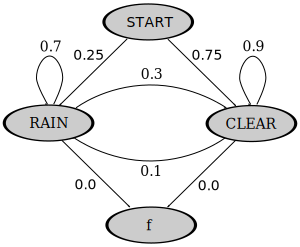
\includegraphics[scale=0.8]{hmm-ex-graph-2}
\end{center}
\end{figure}

I define a number of probabilities associated with an HMM:
\begin{enumerate}
\item The {\it joint probability} $p(x,y\parcond\theta)$ of a observation
  sequence $x$ and state sequence $y$. This is the probability that an
  HMM with parameters $\theta$ will generate the state sequence $y$
  and generate the observation $x_t$ in every state $y_t$.
\item The {\it total probability} $p(x\parcond \theta)$ of an observation
  sequence $x$. This is the probability that the observation sequence
  generated by the HMM is $x$.
\item The {\it conditional probability} $p(y\cond x\parcond\theta)$ of a
  state sequence $y$ given an observation sequence $x$. That is, how
  likely it is that the model passes through the states in $y$ when
  emitting the observations $x$.
\item The {\it marginal probability} $p(z, t\cond x\parcond \theta)$ of
  label $z$ at position $t$ given the observation sequence $x$. FIXME
\end{enumerate}

To formally define these probabilities, let $\theta = \{i,\ T,\ E\}$ be
the set of parameters of some HMM with observation set $X$ and hidden
state set $Y$, $x = (x_1,\ ...,\ x_T) \in X^T$ be a sequence of
observations and $y = (y_1,\ ...,\ y_T) \in Y^T$ a sequence of hidden
states (having the same length as $x$). Then the joint probability
$p(x,y;\theta)$ of $x$ and $y$ given $\theta$ is defined by Equation
\eqref{hmm-joint-prob}.
\begin{equation}
p(x,y\parcond\theta) = i(y_1) \cdot \Bigg( \prod_{t = 1}^{T-1} t_{y_t}(y_{t + 1})\Bigg) \cdot t_{y_T}(f) \cdot \prod_{t = 1}^T e_{y_t}(x_t)\label{hmm-joint-prob}
\end{equation}
Equation \eqref{hmm-joint-prob} is a product of two factors: the
probability of the hidden state sequence $y$, determined by the
initial and transition probabilities, and the probability of the
emissions $x_t$ given hidden states $y_t$ determined by the emission
probabilities.

There is no limit on the number of hidden states in $Y$ that can emit
an observation $x_t$. Therefore, it is quite possible that the same
observation sequence $x$ can be generated from many different state
sequences. The total probability $p(x\parcond\theta)$ of an observation
sequence $x$ can be found by summing over all state sequences that
could have generated $x$. It is defined by Equation
\eqref{hmm-obs-prob}.
\begin{equation}
p(x\parcond\theta) = \sum_{(y_1,\ ...,\ y_T) \in Y^T} p(x, y\parcond \theta)\label{hmm-obs-prob}
\end{equation}

Possibly the most important probability associated to the HMM is the
conditional probability $p(y\cond x\parcond\theta)$ of state sequence $y$
given observations $x$. This is an important quantity because
maximizing $p(y\cond x\parcond\theta)$ with regard to $y$ will give the MAP
assignment of observation sequence $x$. It is defined by Equation
\eqref{hmm-cond-prob}.
\begin{equation}
p(y\cond x\parcond\theta) = \frac{p(x,y\parcond\theta)}{p(x\parcond\theta)}\label{hmm-cond-prob}
\end{equation}

Finally, the marginal probability of state $z$ at position $t$ given
the observation sequence $x$ is computed by summing, or marginalizing,
over all state sequence $y$, where $y_t = z$. It is defined by
Equation \eqref{hmm-marg-prob}
\begin{equation}
p(z, t\cond x\parcond \theta) = \frac{\sum_{(y'_1,\ ...,\ y'_T) \in Y^T, y'_t = z} p(x, y'\parcond \theta)}{p(x\parcond\theta)}\label{hmm-marg-prob}
\end{equation}

\section{Inference}
%\begin{itemize}
%\item The forward algorithm.
%\item Guarding against underflow: Dynamic scaling \citep{Rabiner1989} or exp-sum-log \citep{Durbin1998}.
%\item The Viterbi algorithm.
%\item Fixed beam search.
%\item Determining the beam: fixed, threshold and adaptive beam \citep{pal2006}.
%\item The forward-backward algorithm and multitagging.
%\end{itemize}
Informally, inference in HMMs means finding a maximally
probable sequence of hidden states $y$ that might have emitted the
observation $x$. As \cite{Rabiner1989} points out, this statement is
not strong enough to suggest an algorithm. 

Maximally probable is an ambiguous term when dealing with structured
models. It could be taken to mean at least two distinct things. The
MAP assignment $y_{MAP}$ of the hidden label sequence is the most
probable joint assignment of labels defined by Equation
\eqref{hmm-map}. Another possible definition would be the {\it maximum
  marginal} (MM) assignment. It chooses the most probable hidden
state for each word regardless of the states of all other words. The
MM assignment $y_{MM}$ is defined by Equation \eqref{hmm-mm}.

\begin{equation}
y_{MAP} = \argmax_{y\in Y^T} p(y\cond x\parcond\theta)\label{hmm-map}
\end{equation}

\begin{equation}
y_{MM} = \argmax_{y\in Y^T} \prod_{t = 1}^T p(y_t, t \cond x\parcond\theta)\label{hmm-mm}
\end{equation}

As \cite{Merialdo1994} and many others have noted, the MAP and MM
assignments maximize different objectives. The MM assignment maximizes
the accuracy of correct states per observations whereas the MAP
assignment maximizes the number of completely correct state
sequences. Both objectives are important from the point of view of POS
tagging. However, they are often quite correlated and, at least in
POS tagging, it does not matter in practice which of the criteria is
used \citep{Merialdo1994}.

Most systems, for example \cite{Church1988,Brants2000,Halacsy2007},
have chosen to use MAP inference. MAP inference is probably preferred
because it makes inference easier and is faster in practice. Moreover,
there are inexact variants of MAP inference which are even faster than
exact MAP search. I will elaborate this further in \ref{hmm-viterbi}.

Although, MM inference is more rarely used with HMMs, computing the
marginals is important both in unsupervised estimation of HMMs and
discriminative estimation of sequence models. Therefore, I will
present the relevant algorithm in \ref{hmm-fw-bw}.
 
\subsection{The Forward Algorithm}

\subsection{The Viterbi Algorithm}
\label{hmm-viterbi}

\subsection{The Forward-Backward Algorithm}
\label{hmm-fw-bw}
\section{Estimation}
%\begin{itemize}
%\item Counting vs Baum-Welch.
%\item Smoothing over orders.
%\item Smoothing missing counts.
%\item Estimating parameters for OOV word model.
%\end{itemize}

HMMs can be trained in different ways depending on the quality of the
available data, but also on the task at hand. The classical setting
presented by \cite{Rabiner1989} is nearly completely unsupervised: the
HMM is trained exclusively from observations. Some supervision is
nevertheless usually required to determine the number of hidden
states\footnote{Although methods for determining the number of states
  from the data exist \citep{foo}.}. Additionally priors on the
emission and transitions distributions may be required to avoid
undesirably even distributions
\citep{Cutting1992,Johnson2007}.

The unsupervised training setting has two important and
interrelated applications:
\begin{enumerate}
\item Modeling a complex stochastic process from limited data. Here
  the HMM can be contrasted to a Markov chain \citep[318--320]{Manning1999}, where
  each emission can occur in a unique state leading to a higher degree
  of data sparsity and inability to model under-lying structure.
\item Uncovering structure in data, for example part-of-speech
  induction \citep{Johnson2007}.
\end{enumerate}
The classical method for unsupervised Maximum likelihood estimation of
HMMs is the {\it Baum-Welch algorithm} \citep{Rabiner1989}, which is
an instance of the {\it expectation maximization algorithm} (EM)
\citep{Dempster1977} for HMMs.

\section{HMM taggers and Morphological Analyzers}
\begin{itemize}
\item Limiting transitions.
\item How much of an improvement can be expected?
\end{itemize}


\section{HMMs for POS Tagging}

\section{Problems}
\begin{itemize}
\item Local normalization.
\item Inability to use word context.
\item Label bias.
\item The inability to use rich features, causes problems in domains
  other than POS tagging and in POS tagging for MR languages.
\item Smoothing is difficult.
\item Differences in performance between generative HMMs and
  discriminative approaches are even greater for morphologically
  complex languages and small training sets.
\item OOV words may require different mechanisms depending on
  language again causing problems for MR lanuages.
\end{itemize}

\section{Enriching the emission and transition models}
\begin{itemize}
\item \cite{Halacsy2007} and \cite{Silfverberg2011}.
\end{itemize}


\chapter{Discriminative Models}
\label{chapter:crf}
%\section{Discriminative modeling}

As seen in Chapter \ref{chapter:hmm}, a first order HMM POS tagger can
be viewed as a process which alternates between sampling a word from a
label specific observation distribution and sampling the next
morphological label from a label specific transition distribution. The
emitted word and the next morphological label are conditioned {\it
  solely} on the current morphological label. These independence
assumptions are harsh. For example, collocations cannot be adequately
modeled because the model does not include direct information about
word sequences.

Although information about collocations and orthography is quite
useful in morphological tagging, it is often difficult to incorporate
such information in a generative model. As \cite{Sutton2012} note, two
principal approaches could be attempted:
\begin{enumerate}
\item Extending the emission model presented in Chapter
  \ref{chapter:hmm} to incorporate additional sources of
  information.\label{ap:1}
\item Replacing the usual emission model with a Naive
  Bayes' model which in theory can handle arbitrary
  features.\label{ap:2}
\end{enumerate}

Approach \ref{ap:1} is difficult in a fully generative setting because the
emission model needs to account for the complex dependencies that
exist between sentence level context and orthography. There simply does not
seem to exist a straightforward way of modeling the dependencies.\footnote{Although recent development in deep learning might make this approach viable.}

Approach \ref{ap:2}, that is making the naive Bayes assumption,
corresponds to disregarding the dependencies that exist between
orthography, word collocations and other sources of contextual
information. In the domain of named entity extraction, which is
closely related to morphological tagging, \cite{Ruokolainen2013} show
that approach \ref{ap:2} also fails. In fact the experiments in the
paper indicate that adding richer context modeling such as adjacent
words may worsen the performance of a tagger with a Naive Bayes
emission model. One reason for this may be that the richer sources of
information are often correlated and this violates the independence
assumption of the Naive Bayes model. This can cause it to give overly
confident probability estimates \citep{Sutton2012}. When the emission
probabilities are over confident, and thus biased, combining them with
the transition model can be problematic.

In contrast to generative sequence models, discriminative sequence
models such as Maximum Entropy Markov Models \citep{Ratnaparkhi1998}
and Conditional Random Fields \citep{Lafferty2001} can incorporate
overlapping sources of information. They model the conditional
distribution of label sequences $p(y\cond x)$ directly instead of
modeling the joint distribution $p(x,\ y)$. Therefore, they do not
need to model dependencies between words and orthographic features.

Discriminative models assign probabilities $p(y\cond x)$ for label
sequences $y = ({\rm DT},\ {\rm NN},\ {\rm VBZ},\ {\rm .})$ and word sequences $x = ({\rm The},\ {\rm dog},\ {\rm eats},\ {\rm .})$ by extracting {\it features} from
the input sentence and label sequence. Examples of features
include {\bf the current word is ``dog'' and its label is NN} and {\bf the previous label is DT and
  the current label is NN}. Each feature is associated with a parameter value and the
parameter values are combined to give the conditional likelihood of
the entire label sequence. Naturally, the label sequence which
maximizes the conditional likelihood given sentence $x$ is the label
sequence returned by the discriminative POS tagger.

In generative models, emissions and transitions are independent. Both
are determined exclusively based on the current label. In contrast,
there are no emissions or transitions in a discriminative
model. Instead, it is customary to speak about unstructured features
which relate the label in one position to the input sentence, and
structured features, which incorporate information about the label
sequence. Simplifying a bit, discriminative models make no
independence assumptions among features relating to a single position
in the sentence. This allows for improved fit to training data but
parameter estimation becomes more complex as we shall soon
see. Moreover, discriminative models are more prone to
over-fitting.\footnote{This is of course an example of the famous bias-variance
trade-off \citep{Geman1992}.}


%\section{Maximum Entropy Modeling}
%\label{sec:me}

%\paragraph{Example}
%\label{sec:maxent-ex}

\section{Basics}
\label{crf:basics}

In this section, I will describe a CRF POS tagger from a practical
point-of-view. The tagging procedure encompasses two stages: feature
extraction and inference using an exact or approximate inference
algorithm. Inference in CRFs is very similar to inference in HMMs. We
did not discuss feature extraction in association to HMMs. The
discussion was omitted because HMM taggers use a fixed set of features
(the current word and preceding labels). In contrast, CRF taggers can
incorporate a variety of user defined features.

As seen above, features are true logical propositions that apply to a
position $t$ in a labeled sentence. They connect aspects of the input
sentence to the label at position $t$.\footnote{Although the original
  first order CRF formulation by \cite{Lafferty2001} allows for
  features that refer to both unstructured and structured information
  at the same time, the author has found that such features do not
  improve model performance significantly. They, however, do increase model
  size substantially. Therefore, the models used in the thesis extract
  purely unstructured features, which relate one label to the
  sentence, and structured features, which only relate adjacent labels
  to each other.} %Given
%sentence $x$ and label sequence $y$ of length $n$, we extract features
%at every position $t$ in the sentence. For example at position $2$ in
%sentence $x$, we could extract {\it The current word $x_t$ is ``dog''
%  and the label is ``NN''} and {\it The previous label is ``DT'' and
%  the current label is ``NN''}. We could, however, not extract the
%same feature {\it The current word is ``dog'' and the label is ``NN''}
%at position $1$, because this proposition is false when $t = 1$ (the
%word at position 1 is ``The'' and the label is ``VBZ'').
They consist of two components: a feature template, for example {\bf
  The current word is ``dog''} or {\bf the previous label is DT}, and
a label {\bf the current label is NN}. The set of features recognized
by a CRF POS tagger consists of all conjunctions $f \& y$ of a feature
template $f$ and label $y$. For example, the feature {\bf The current
  word is ``dog'' and the current label is DT} can be formed although
it is unlikely that this feature would ever be observed in actual
training data.

\cite{Ratnaparkhi1996} introduced a rather rudimentary feature set and
variations of this feature set are commonly used in the literature
(for example \cite{Collins2002}, \cite{Lafferty2001}, and Publications \ref{pub:5} and \ref{pub:6}). Let $W$ be
the set of word forms in the training data. Additionally let $P$ and
$S$ be the sets of prefixes and suffixes of maximal length $4$ of all
words $w \in W$. Then, the Ratnaparkhi feature set contains the
unstructured feature templates in Table \ref{tab:uratna} and the
structured feature templates in Table \ref{tab:sratna}.

\begin{table}[!htb]
\begin{tabular}{ll}  
Feature template & Example\\
\hline
The current word is $w \in W$ & The current word is ``dog''\\
The current word has prefix $p\in P$ & The current word has prefix ``d-''\\
The current word has suffix $s\in S$ & The current word has suffix ``-og''\\
The current word contains a digit & \\
The current word contains a hyphen & \\
The current word contains an upper case letter & \\
The previous word is $w \in W$ & The previous word is ``The''. \\
The next word is $w\in W$ & The next word is ``eats''. \\
The word before the previous word is $w$ & \\
The word after the next word is $w$ & \\
\end{tabular}
\caption{The set of unstructured feature templates introduced by \cite{Ratnaparkhi1996}}\label{tab:uratna}
\end{table}

\begin{table}[!htb]
\begin{tabular}{ll}
Feature template & Example\\
\hline
The label of the previous word is $y$ & The label of the previous word is ``NN''. \\
The label of the previous two words are $y'$ and $y$ & The labels of the two previous words are\\
 & ``DT'' and ``NN''. 
\end{tabular}
\caption{The set of structured feature templates introduced by \cite{Ratnaparkhi1996}}\label{tab:sratna}
\end{table}

As in the case of an HMM, the order of a CRF can be increased. This
corresponds to including more label context in structured features. It
is instructive to estimate the number of features when using a
realistic training set. It is
$|\mathcal{Y}|^3 + |\mathcal{F}||\mathcal{Y}|$, where $\mathcal{Y}$ is
the set of morphological labels and $\mathcal{F}$ is the set of
unstructured feature templates.

For small label sets and large training data, the bulk of all features
consists of unstructured features. However, for large
label sets in the order of $1,000$ labels, there will be a significant
number of structured features (one billion in this case). This
necessitates either dropping second order structured features or using
sparse feature representations. All structured features simply cannot
be represented in memory. We will see techniques to circumvent these
problems. Especially the averaged perceptron is essential.

It is common to represent the CRF using linear algebra. Each position
$t$ in the sentence is represented as a vector $\phi_t$ whose
dimensions correspond to the entire space of possible features. The
selection of features is finite because it is limited by the training
data. There are only finitely many word forms, suffixes, morphological
labels and so on in the training data. The elements of each vector
$\phi_t$ represent activations of features. In the present work all
elements are either $0$ or $1$ mirroring the truth value of a feature
at position $t$ in the labeled sentence. Other activations in
$\mathbb{R}$ can also be used when appropriate.

In order to represent sentence positions as vectors, we need an
injective index function $I$ which maps features onto consecutive
integers starting at 1. For each feature $f$, $I(f)$ will correspond
to one dimension in $\phi_t$. In a concrete implementation of a CRF
tagger, features can be represented as strings and the index function
$I$ can be implemented as a hash function.
 
Given a sentence $x$ and label sequence $y$, we can extract the set of features
$F_t(x)$ for each position $t$ in $x$. Let $\phi_t \in \mathbb{R}^N$ be a vector defined by
$$\phi_t(i) = 1,\ {\rm\ if}\ i \le N\ {\rm and}\ I(f) = i\ {\rm for\ some\ }f\in F_t$$
all other entries in $\phi_t$ are $0$. 

Given a parameter vector $\omega \in \mathbb{R}^N$, the probability $p(y|x)$ is
$$p(y|x) \propto \prod_{t = 1}^T \exp(\omega^\top \phi_t)$$
Specifically, the same parameter vector $\omega$ is shared by all
sentence positions and the probability $p(y|x)$ is a log linear
combination of parameter values in $\omega$.

\section{Logistic Regression}
%\begin{itemize}
%\item Detailed view of logistic regression. 
%\item Relation to maximum entropy.
%\item Why are MEMMs not better than HMMs?
%\item Label and observation bias.
%\end{itemize}

The simplest Conditional Random Field is the {\it Logistic Regression
  Model}. It is an unstructured probabilistic discriminative
model. In this section, I will present a formal treatment of the
logistic regression model because it aids in understanding more general
CRFs.

Regular linear regression models a {\it real valued quantity} $y$ as a
function of an input $x = (x_1, ..., x_n)$. In contrast, the logistic
regression model models {\it the probability} that an observation $x$
belongs to {\it a class} $y \in |\mathcal{Y}|$, where $\mathcal{Y}$ is
a finite set of classes. For example, a logistic classifier can be
used to model the probability of a tumor belonging to the class {\sc
  MALIGNANT} or BENIGN. The probability is based on quantifiable
information about the tumor such as its size, shape. These quantifiable
sources of information are the {\it feature templates} of the logistic
classifier and combined with class labels they constitute the features of
the
model. %In concrete terms, let $f$ be the feature template {\it Tumor diameter greater then 5 cm} and $y$ be the class MALIGNANT, then we can form a feature $f \& y$ ``{\it Tumor diameter greater than 5 cm} and the tumor is MALIGNANT''.

The material at hand deals with linguistic data where most information
sources are binary, for example whether a word ends in suffix ``-s''
and whether a word is preceded by the word ``an''. In other domains
such as medical diagnostics, more general features can be used. These
can be real valued numerical measurements such as the diameter of a
tumor. This treatment of logistic classifiers will assume binary
feature activations. When using binary features, we can equate the example $x$
with the set of feature templates $F_x \subset \mathcal{F}$ that it {\it
  activates}, that is {\bf Tumor diameter $\geq$ 5 cm}, {\bf The previous word is ``an''} and so on. Examples that activate the exactly same
feature templates will be indistinguishable from the point of view of the
Logistic Regression model.

The logistic classifier associates each combination of a feature
template and class with a unique feature and a corresponding real
valued parameter. Intuitively, the logistic classifier models
correlations of feature templates and classes by changing the
parameter values of the associated features. For example, it might
associate the feature template {\bf Tumor diameter $\geq$ 5 cm} more
strongly with the class MALIGNANT than the class BENIGN if large
tumors are cancerous more often than smaller ones. This could be
reflected in the parameter values of the model that correspond to the
features $f =$ {\bf Tumor diameter $\geq$ 5 cm and class is MALIGNANT}
and $f' =$ {\bf Tumor diameter $\geq$ 5 cm and class is BENIGN} so
that the parameter value for $f$ is greater than the parameter value
for $f'$. In general parameter values, however, also depend on other
features and feature correlations in the model. Therefore we can say
that the parameter value of, $f$ will be guaranteed to be greater than
the parameter value of $f'$ when $f$ is the sole feature template and
the model accurately reflects the original distribution of class
labels among examples. In the general case, where there are several
feature templates, this might fail to hold.

Formalizing the notation used in Section \ref{crf:basics}, let $\mathcal{F}$ be
a finite set of feature templates and $\mathcal{Y}$ a finite set of
classes. Each combination of feature template $f \in \mathcal{F}$ and class $y
\in \mathcal{Y}$ corresponds to a unique feature. Therefore, the model will have
$|\mathcal{F} \times \mathcal{Y}|$ features in total. Let $\theta \in \R^{|\mathcal{F} \times \mathcal{Y}|}$ be a real valued
parameter vector and let ${\mathrm I}$ be a
1-to-1 index function which maps each feature onto and index of $\theta$, that is $1 \leq {\mathrm I}(f,
y) \leq |\mathcal{F} \times \mathcal{Y}|$.

For each example $x$, let $F_x \subset \mathcal{F}$ be the set of feature templates that $x$ activates and let $y \in \mathcal{Y}$ be a class. Then the feature vector associated with $x$ and $y$ is $\phi(x,y) = \{0, 1\}^{|\mathcal{F} \times \mathcal{Y}|}$ defined by
\[
  \phi(x,y)_i = \left\{
  \begin{array}{ll}
  1 & {\rm iff\ } i = {\mathrm I}(f,y) {\rm\ for\ some\ }f \in F_x{\rm,} \\ 
  0 & {\rm otherwise.}  
  \end{array}
  \right.
\]

%$$F_y(I(f, y)) = 1\ {\rm iff\ }f \& y\ {\rm is\ true}.$$

Now the conditional probability $p(y\cond x)$ defining the Logistic
classifier is given by Equation \eqref{eq:logistic}. The equation
defines a probability distribution over the set of classes
$\mathcal{Y}$ because each quantity $p(y\cond x\parcond\theta)$ is a
positive real and the quantities sum to 1.

\begin{equation}
p(y\cond x\parcond \theta) = \frac{\exp(\theta^\top \phi(x,y))}{\sum_{z \in Y}\exp(\theta^\top \phi(x,z))}\label{eq:logistic}
\end{equation}

\paragraph{Inference} Inference for a Logistic Regression Model
corresponds to performing the maximization in Equation \ref{eq:logistic,inference}. As the equation demonstrates, the full computation of the probability is not required when classifying. The maximization can be performed without normalization.

\begin{equation}y_{max} = \argmax_{y \in Y} p(y\cond x\parcond \theta) = \argmax_{y\in Y} \frac{\exp(\theta^\top \phi(x,y))}{\Z(x;\theta)} = \argmax_{y \in Y} \exp(\theta^\top \phi(x,y))\label{eq:logistic,inference}\end{equation}

To avoid underflow when using finite precision real numbers (such as
floating-point numbers), the maximization is usually rephrased as the
minimization of a loss function in Equation
\ref{eq:logistic,inference,log} by applying a logarithmic
transformation $x \mapsto -\log(x)$.

\begin{equation}y_{min} = \argmin_{y\in Y} -\theta^\top \phi(x,y)\label{eq:logistic,inference,log}\end{equation}

From a practical implementation perspective, the minimization in
Equation \ref{eq:logistic,inference,log} boils down to computing one
inner product $\theta^\top \phi(x,y)$ for each label $y \in Y$ and
finding the minimum. Using a suitable sparse approach each of the
inner products can be computed in $\O(|F_x|)$ time, where $F_x$ is the
set of feature templates activated by example $x$. Therefore, the
worst-case complexity of classification is dependent on the size of
the label set $Y$ and the number of feature templates $f \in F$, that
is the complexity is $\O(|Y||F|)$.

\paragraph{Estimation}
The Logistic Regression Model is log-linear as demonstrated by
Equation \ref{eq:logistic,log}, which represents the model using a
loss function $\mathcal{L}$.

\begin{equation}
\mathcal{L}(\theta\parcond\mathcal{D}) = -\log p(y\cond x\parcond \theta) = log(\Z(x;\theta)) - \theta^\top F_y(x)\label{eq:logistic,log}
\end{equation}
Here $Z(x;\theta) = \sum_{z \in Y}\exp(\theta^\top F_{z}(x))$ is the partition function for example $x$.

Given labeled training data $\data = \{(x_1,\ y_1),\ ...,\ (x_n,\
y_n)\}$, there exist several options for estimating the parameters
$\theta$. The most commonly used is {\it empirical risk minimization},
which finds a parameter vector that minimizes the loss $\mathcal{L}$ on the
training data $\mathcal{D}$ as shown in Equation \eqref{eq:logistic,ml}.

\begin{equation}
\theta = \argmin_{\theta'} \mathcal{L}(\theta\parcond \mathcal{D}) = \argmin_{\theta'}\sum_{(x,\ y) \in \mathcal{D}} \Z(x\parcond \theta) - {\theta'}^\top F_y(x)\label{eq:logistic,ml}
\end{equation}

The probability $p(y\cond x\parcond \theta)$ has exponential form,
which means that the probability is proportional to a product of
factors of the form $e^{ap}$, where $a$ is an activation (0 or 1) and
$p$ is a parameter. This has three important consequences:

\begin{enumerate}
\item The function $\theta \mapsto p(y\cond x\parcond \theta)$ is smooth.
\item The function $\theta \mapsto p(y\cond x\parcond \theta)$ is convex.
\item There exists a {\it unique} $\theta$ maximizing the likelihood of the training data $\mathcal{D}$.\footnote{Technically this requires that the possible values of $\theta$ are limited into a compact subset of the parameter space.}
\item The model $p(y\cond x\parcond \theta)$ is maximally unbiased. 
\end{enumerate}

Smoothness follows from the fact that each factor $a \mapsto e^{ap}$
is smooth and products and sums of smooth functions are
smooth. Convexity of the likelihood follows by a straightforward application of the Hölder inequality \cite{}. Property 3 is a consequence of properties 1 and 2.
Property 4 is discussed in \cite{foo}.

Although the maximization in Equation \ref{eq:logistic} cannot be
solved exactly in general, the convexity and smoothness of
$p(y\cond x\parcond \theta)$ mean that efficient numerical methods can
be used for approximating the maximum.

Gradient based methods such as SGD (leading to online estimation) and
L-BFGS (leading to batch estimatiom) require information about the
partial derivatives of the loss function. Therefore the partial
derivatives $\partial\mathcal{L}(\theta\parcond
\mathcal{D})/\partial\i$ need to be computed. Examining Equation
\ref{eq:logistic,ml}, we can see that the loss consists of two terms
$f(\theta\parcond \mathcal{D}) = \log(\Z(\mathcal{D}\parcond \theta))$
and $g(\theta\parcond\mathcal{D}) = \sum_{(x,y) \in
  \mathcal{D}}\theta^\top F_y(x)$. The partial derivative of $g$
w.r.t. parameter $i$ can be computed in the following way
$$\frac{\partial g}{\partial i} = \sum_{(x,y) \in \mathcal{D}} F_y(x)[i]$$
This quantity represents the total activation of feature $i$ in the training data and is called {\it the observed count} of feature $i$. 

Using the chain rule of derivatives, we get the partial derivative of $f$ w.r.t. to param $i$
$$\frac{\partial f}{\partial i} = \sum_{(x,y) \in \mathcal{D}} \frac{\sum_{y' \in \mathcal{Y}}F_{y'}(x)[i] \exp(\theta^\top F_{y'}(x))}{\Z(x\parcond\theta)} = \sum_{(x,y) \in \mathcal{D}} \sum_{y' \in \mathcal{Y}}F_{y'}(x)[i] p(y'|x\parcond\theta)$$
This is the {\it expected count} of feature $i$ which is the
activation of feature $i$ in the data set $x_1, ...,x_n$ predicted by
the model given all possible label assignments.

Using the partial derivatives of the functions $f$ and $g$, we see that the gradient of the loss function $\mathcal{L}$ is defined by
\begin{equation}\nabla \mathcal{L}[i] = \sum_{(x,y) \in \mathcal{D}} \Big( \sum_{y' \in \mathcal{Y}}F_{y'}(x)[i] p(y'|x\parcond\theta) \Big) - F_y(x)[i] \label{eq:reg-loss}\end{equation}
Equation \ref{eq:reg-loss} shows that the loss is zero when the
expected and observed counts for each feature agree.\footnote{As each feature $i$ is label specific in the current work, the sum $\sum_{y' \in \mathcal{Y}}F_{y'}(x)[i] p(y'|x\parcond\theta)$ reduces to $F_y(x)[i] p(y|x\parcond\theta)$. It is thus easy to see that the loss vanishes if $p(y|x\parcond\theta) = 1$ for each $(x,y)\in\mathcal{D}$.} The
properties for the logistic regression model discussed above guarantee
that this there is at most one $\theta_{ML}$ like this and, when it
exists, $\theta_{ML}$ is the maximum likelihood estimate for the
parameters.

Regularization methods such as $L_1$ and $L_2$ introduced in Chapter
\ref{chap:ml} can also be applied to the model. This naturally changes
the gradient and also the properties of the model. Analysis of the
regularized model falls outside of the scope of this thesis.

\section{The Perceptron Classifier}
\label{sec:perc}

The perceptron algorithm \citep{Rosenblatt1958} is an alternative to
empirical risk minimization for learning the weights of a
discriminative classifier. As seen above, the logistic classifier
optimizes the conditional probability of gold standard classes given
training inputs. In contrast, the perceptron rule directly optimizes
the classification performance of the discriminative classifier. 

Intuitively, the multi-class perceptron algorithm works by labeling
each training example in order using a current estimate of the
parameter vector $\theta$ and adjusting the parameter vector whenever
training examples are incorectly labeled. Consequently, the perceptron
algorithm is an online learning algorithm.

\paragraph{Inference} Similarly as in the case of any linear
classifier, the perceptron classifier scores each example $x$ and class $y$ by
$\theta^\top\phi(x,y)$. Example $x$ is labeled by the $y \in \mathcal{Y}$ which maximizes the score.

% which is computed using the current estimate of
%the parameter vector. 
%If the score of the gold standard class
%$y_{gold}$ is not the highest one, that is there is a class $y$ which
%scores higher or equally high, then the parameter vector $\theta$ is
%modified in a way which increases the score for the gold standard
%class and decreases the score for the highest scoring class $y$.

\paragraph{Estimation} The perceptron algorithm is an error-driven
online learning algorithm. When a classification error is encountered
during estimation, that is $\theta^\top\phi(x,y) >
\theta^\top\phi(x,y_{gold})$ for some $y \ne y_{gold}$, the parameter vector $\theta$ is
adjusted for relevant features. For every feature template $f$ which
is activated by the example $x$, the weights $\theta[I(f, y_{gold})]$
and $\theta[I(f, y)]$ are adjusted. Here $I(f, y_{gold})$ and $I(f,
y)$ are the features corresponding to the template $f$ and classes
$y_{gold}$ and $y$, respectively. The perceptron rule for weight
adjustment is the following:
$$\theta[I(f, y_{gold})] = \theta[I(f, y_{gold})] + 1 {\rm\ and\ }\theta[I(f, y)] = \theta[I(f, y)] - 1$$

\begin{algorithm}[!p]
\begin{center}
\caption{The pass of the perceptron algorithm in Python 3.}\label{forward-algorithm}
\begin{lstlisting}[linewidth=\textwidth]
def infer(x, fextractor, theta, label_set)
    """
        x          - An observation.
        fextractor - A vector valued function. 
                     len(fextractor(x,y)) == len(theta). 
        theta      - A parameter vector.
        label_set  - Set of potential labels. 
    """
    sys_label = None
    max_score = -float('inf')
 
    for y in label_set:
        score = dot_product(theta, fextractor(x,y))
        if score > max_score:
            max_score = score
            sys_label = label

    assert(sys_label != None)
    return sys_label

def perceptron(data, fextractor, theta, label_set): 
    """
        data       - data[i][0] is an observation, data[i][1] a label.
        fextractor - A vector valued function. 
                     len(fextractor(x,y)) == len(theta) 
        theta      - The parameter vector.
        label_set  - Set of potential labels. 

        Run one pass of the perceptron algorithm.
    """

    for x, y_gold in data:
         y_system = infer(x, fextractor, theta, label_set)
         
         if y_system != y_gold:
             for f in fextractor(x, y_system):
                 theta[f] -= 1
             for f in fextractor(x, y_gold):
                 theta[f] += 1
\end{lstlisting}
\end{center}
\end{algorithm}

The perceptron adjustment does not guarantee that example $x$ is
correctly classified. However, it does guarantee that the score
difference between the gold class and erroneous class decreases.\footnote{There are refinements of the perceptron algorithm, such as the passive-aggressive learning algorithm, which aim to make fewer updates by updating more aggressively when the difference in scores between the erroneous class and gold class is large \citep{Crammer2006}} Given
training data consisting of just one example, it is easy to see that
the perceptron algorithm will eventually classify the example
correctly. If there are more examples, it may however happen that a
correct parameter vector is never found.

The perceptron algorithm {\it converges} when no example in the
training data causes a change in the parameter vector
$\theta$. Equivalently, the perceptron algorithm correctly classifies
every example in the training data. It can be showed that the
perceptron algorithm converges whenever there exists a parameter vector
that correctly classifies the training data \citep{Freund1999}. Such a
data set is called linearly separable. The term originates from a
geometrical interpretation of the 2-class perceptron algorithm, where
the parameter vector defines a hyper plane in the feature space which
divides the space into two halves. A data set is called separable if
there is a hyper space which separates the examples in each of the
classes into their own half space.

When a data set is linearly separable, there are typically infinitely
many parameter vectors that that classify the data set correctly. The
perceptron algorithm will give one of these. Other algorithms exist
which attempt to find an optimal parameter vector in some sense
(e.g. Support Vector Machines \citep{Cortes1995}). These, however,
fall beyond the scope of the present work.

Even when the training set is not linearly separable, the perceptron
algorithm will have good performance in practice. In the non-separable
case, a held out development set is used. Training is stopped when the
performance of the classifier on the development set no longer
improves.

\paragraph{Voting and Averaging} Because the perceptron algorithm
makes fixed updates of size $1$, the parameter vector tends to change
too rapidly at the end of the training procedure. To avoid this, it is
customary to use the average of all parameter vectors from the
training procedure instead of the final parameter vector. This will
give better performance during test time. Parameter averaging is an
approximation of so called {\it voting perceptron}. In voting, each
parameter vector is considered a separate classifier and the
classification is performed by taking a majority vote of all of the
classification results. This is impractical, because there are
thousands of classifiers. Therefore, averaging is used in order to
achieve approximately the same effect.%almost the same effect.

\section{CRF -- A Structured Logistic Classifier}\label{sec:crf}

This Section presents Linear Chain Conditional Random Fields
(CRF).\footnote{More general CRF models can be formulated but these
  mostly fall beyond the scope of this thesis. See \citep{Sutton2012}
  for further details.} Just as the HMM is a structured equivalent of
the NB classifier, the CRF is the structured equivalent of the
logistic regression model. Consequently, many of the algorithms required to run a CRF
tagger are similar to the algorithms required to run an HMM
tagger. Estimation of model parameters is, however, different because
of the discriminative nature of the model.

Another major difference between an HMM classifier and a CRF
classifier is that the CRF classifier typically employs a much larger
set of features. This increases the size of the model. It also makes
the discriminative tagger slow in comparison to the generative
tagger. The slowdown is demonstrated by the experiments in
Publication \ref{pub:6}. However, the accuracy of the discriminative
model in morphological tagging is superior to the generative HMM tagger.

Intuitively, the CRF model resembles a sequence of logistic regression classifiers
with shared parameters. Given a sentence $x = (x_1,\ ...,\ x_T)$,
label sequence $y = (y_1,\ ...,\ y_T)$ and parameters $\theta$ for the
logistic regression model, a score for the label $y_i$ in position $t$ $s(x, y_{t-2},
y_{t-1}, y_t, t\parcond \theta)$ can be computed. Here the logistic regression model
utilizes the input sentence $x$ as well as labels $y_{t - 2}$, $y_{t-1}$ and
$y_t$ to extract unstructured and structured features from the
sentence and label sequence. The score $s$ takes on a familiar form
$$s(x, y_{t-2}, y_{t-1}, y_t, t\parcond \theta) = \exp(\theta^\top F_y(x, t, y_{t-2}, y_{t-1}))$$
where $F_y$ is a vector valued feature extraction function. Each
feature associated to the label $y$ corresponds to one element of the
vector $F_y(x, t, y_{t-2}, y_{t-1})$. Since $F_y$ refers to a context
spanning three labels, the model is a second order model. All
discriminative taggers discussed in this Chapter are assumed to be
second order model. As in the case of the logistic regression model,
each entry of the vector can be an arbitrary real number but in this
thesis they will always be either $0$ or $1$.

The probability of label sequence $y \in \mathcal{Y}^T$ given a sentence $x$ of length $T$ is
\begin{equation}\label{eq:crf}p(y|x\parcond\theta) \propto \prod_{t = 1}^T s(x, y_{t-2}, y_{t-1}, y_t, t\parcond \theta)\end{equation}
In Equation \ref{eq:crf}, the labels $y_{-1}$ and $y_0$ are special
stop labels which do not belong to the label set $\mathcal{Y}$. The partition function of the sentence $x$ is given by
\begin{equation}\sum_{y\in \mathcal{Y}^T}\prod_{t = 1}^T s(x, y_{t-2}, y_{t-1}, y_t, t\parcond \theta)\end{equation}

It is noteworthy, that the probability in Equation \ref{eq:crf} is
normalized for {\it the entire sentence}, not for each position in
isolation. A similar model, where normalization happens in each
position is called the Maximum Entropy Markov Model (MEMM). It has
been shown to give inferior performance in POS tagging of English
\citep{Lafferty2001}.\footnote{The inferior performance of the MEMM
  has been thought to be a result of the so called label bias problem
  \citep{Lafferty2001} although {\it observation} bias may be more
  influential in POS tagging \citep{Klein2002}.}

\paragraph{Inference} Tagging of a sentence using the CRF model is
very similar to HMM tagging. The major difference is that there are
far more features in a CRF model which slows down inference compared
to a typical HMM tagger. As in the case of an HMM, the Viterbi
algorithm has to be used to find the MAP assignment of the label
sequence because of the structured nature of the model. The
forward-backward algorithm can be used to compute the marginal
probabilities of labels.

\paragraph{Estimation} Estimation of the CRF model parameters is more
involved than the straightforward counting which is sufficient for HMM
training. Estimation is instead very similar to estimation of the
logistic regression model parameters. However, the structured nature
of the CRF model complicates matters slightly.

Let $(x, y)$ be a labeled sentence. The observed count of feature $i$ in position $t$ is $F_{y}(x, t, y_{t-2},y_{t-1},y_t)[i]$ and its expected count is
%$$\frac{\sum_{y' \in \mathcal{Y}^T}F_y(x, t, y_{t - 2}', y_{t-1}', y_t')[i] 
%%\exp(\theta^\top F_y(x, t, y_{t - 2}', y_{t-1}', y_t'))
%s(x, t, y_{t-2}', y_{t-1}', y_t')}{\Z(x\parcond\theta)}$$
$$\sum_{y' \in \mathcal{Y}^T} F_y(x, t, y_{t - 2}', y_{t-1}', y_t')[i] p(y'\cond x \parcond \theta)$$
The partial derivative w.r.t. to the loss $\mathcal{L}$ is the difference between the expected and observed counts as in the case of logistic regression.
$$\frac{\partial\mathcal{L}}{\partial i} = \sum_{t=1}^T \Big( \sum_{y' \in \mathcal{Y}^T} F_y(x, t, y_{t - 2}', y_{t-1}', y_t')[i] p(y'\cond x \parcond \theta)\Big) - F_{y}(x, t, y_{t-2},y_{t-1},y_t)[i]$$ 
The quantities $\sum_{y' \in \mathcal{Y}^T} F_y(x_l, t, y_{t - 2}',
y_{t-1}', y_t')[i] p(y'\cond x \parcond \theta)$ have to be computed using
the forward backward algorithm because a naive algorithm has too high computational cost. The need of the forward backward algorithm is the
most important difference between logistic regression and CRF estimation.  Commonly,
the SGD algorithm and L-BFGS are used for the optimization of $\theta$
\citep{Vishwanathan2006}. As in the case of logistic regression model, the CRF model
can also be regularized using for example L1 or L2 regularization
\citep{Sutton2012}.

Held out development data is commonly used to set the number of
training epochs, model order and regularization hyper-parameters.

\paragraph{Alternative estimators} In addition to the ML estimator, a
variety of estimators are available for discriminative taggers. These
alternative estimators are predominantly used because ML estimation
can be quite resource intensive. A commonly used substitute for the ML
estimator is the structured variant of the averaged perceptron
algorithm described in Section \ref{sec:prec-tagger} and taggers
trained using the averaged perceptron algorithm are often called
perceptron taggers (see for example \cite{Collins2002}). Other
examples mentioned by \cite{Sutton2012} are the pseudlikelihood
\cite{Besag1975} and piecewise pseudolikelihood estimators
\cite{Sutton2007}. Publication \ref{pub:4} investigates a
pseudolikelihood inspired variant of the perceptron estimator.

Given a training example $(x,y) \in \mathcal{D}$ where $x = x_1, ..., x_T$ and $y = y_1, ..., y_T$, the pseudolikelihood of $y$ given $x$ is given by equation \ref{eq:pl}. The notation $y_{\neg t}$ in Equation \ref{eq:pl} refers to all the labels in $y$ except label
$y_t$. 
\begin{equation}\label{eq:pl}\prod_{t = 1}^T p(y_t | x, i, y_{\neg t} \parcond \theta)\end{equation}

The complexity of optimizing the parameters $\theta$ with regard to pseudolikelihood is linear linear with regard to sentence length. In contrast, ML estimation which requires the forward-backward algorithm is has quadratic complexity.
This means that the pseudolikelihood estimator is substantially more efficient than ML estimation. However, it
may result in poor accuracy as indicated by the experiments in Publication \ref{pub:4}.


\section{The Perceptron Tagger}
\label{sec:prec-tagger}

Whereas the unstructured perceptron classifier presented in Section
\ref{sec:perc} is a discriminative classifier similar to the logistic
regression model except that it uses perceptron estimation, a
perceptron tagger \citep{Collins2002} is a sequence labeling model
similar to the CRF except that it uses perceptron estimation.

The model is formulated very similarly as the CRF model. It also uses
a real valued parameter vector $\theta$ but the definition of the score of a label sequence $y$ given sentence $x$ is different 
\begin{equation}s(y|x\parcond\theta) = \sum_{i = 1}^T s(x, y_{i-2},
  y_{i-1}, y_i, i\parcond
  \theta)\label{eq:perc-classifier}\end{equation} The definition of
the score $s$ in an individual position $t$ in Equation
\ref{eq:perc-classifier} is defined as $s(x, y_{i-2}, y_{i-1}, y_i,
i\parcond \theta) = \theta^\top F_y(x, i, y_{i-2}, y_{i-1})$, where
$F_y$ is the vector valued feature extraction function for label
$y$. The definition of the perceptron model is simpler than the
definition of the CRF model. The reason is that the perceptron model
is not intended for defining a probability distribution among label
sequence. It can only be used for determining the best label sequence
with regard to a sentence $x$.

\paragraph{Inference} The Perceptron tagger uses the Viterbi algorithm
for exact inference. Beam search can be used for faster approximate
inference together with a label dictionary as shown in Publication
\ref{pub:6}. Chapter \ref{chapter:finnpos} presents experiments on
varying beam widths.

\paragraph{Estimation}Whereas, CRF estimation requires the
forward-backward algorithm, perceptron estimation only requires the
Viterbi algorithm.  Exactly as in the case of the unstructured perceptron
algorithm, each training example (i.e. sentence) is labeled and
unstructured and structured features are updated accordingly. The
number of training epochs is determined using held-out data. As in the
case of the unstructured perceptron algorithm, parameter averaging is
useful for improving the accuracy of the percetron tagger.

Besides the standard perceptron algorithm, there are many
approximative perceptron variants. Publication \ref{pub:4} introduces
the pseudopeceptron and piece-wise pseudoperceptron estimators which
are inspired by the pseudolikelihood and piecewise pseudolikelihood
estimators for the CRF model. In the spirit of pseudolikelihood, the
pseudoperceptron maximizes the score of each label in isolation as shown by equation \ref{eq:pp}. The
remaining labels in the sentence are fixed to their gold standard
values.
\begin{equation}\label{eq:pp}
s(y|x,y_{gold}\parcond\theta) = \sum_{t=1}^T s(y|x,y_{gold,\neg t}\parcond \theta).
\end{equation}

\paragraph{Beam search for estimation} A high model order and large
label set can result in a prohibitive runtime for the Viterbi
algorithm.  It has a time complexity that is dependent on the $n +
1$st power of the label set size for an $n$th order model. This
problem can be avoided using beam search during estimation instead of
the Viterbi algorithm. This reduces the complexity to
$O(T|\mathcal{Y}|b$, where $T$ is the size of the training data,
$\mathcal{Y}$ the label set and $b$ is the beam width.

Because beam search is an approximative inference algorithm, it may
however not give the correct MAP assignment for a sentence. It may
happen that beam search returns a label sequence $y_{sys}$ for
training sentence $x$ whose score with regard to the current model
parameters is lower than the score of the gold label sequence
$y_{gold}$. This leads to perceptron updates which are not necessary
because the model would already correctly label sentence $x$, if only exact
inference were used. In some domains such as syntactic parsing, this
leads to significant reduction in classification performance
\citep{Huang2012}

\paragraph{Violation fixing} To avoid superfluous perceptron updates,
a technique called violation fixing can be used \citep{Huang2012}
(this is an extension of the early update technique suggested for
incremental parsing in \cite{Collins2004}). \cite{Huang2012} suggest
several related violation fixing methods. The essence of the methods
is to compute the score for each prefix of the label sequence
$y_{sys}$ returned by beam search and each prefix of the gold standard
label sequence $y_{gold}$. One prefix length $i$ is then selected so
that the score of $y_{sys}[1:i]$ is higher than
$y_{gold}[1:i]$.\footnote{If such an $i$ does not exist, then the
  score for $y_{sys}$ is in fact higher than the score of $y_{gold}$.}
Updates are then performed for $y_{sys}[1:i]$ and $y_{gold}[1:i]$. The
choice of $i$ depends on the violation fixing method. For example, the
maximum violation criterion corresponds to choosing an $i$ which
maximizes the score difference between $y_{sys}[1:i]$ and
$y_{gold}[1:i]$.

In the experiments presented in Publication \ref{pub:6}, violation
fixing did not result in consistent statistically significant
improvements. It may be that violation fixing is more influential in
parsing than POS tagging or morphological tagging.

\begin{itemize}
\item Hierarchical CRF \cite{Muller2013}, \cite{Weiss2010} and \cite{Charniak2005}.
\end{itemize}

\paragraph{Cascaded Model Architecture} Beam search can be used to
speed up estimation for the perceptron tagger. For large label sets,
even beam search may not lead to sufficient run-time optimization
because the complexity of beam search is dependent on the label set
size. Publication \ref{pub:6} introduces a method to optimize
estimation even further by only considering a subset of $\mathcal{Y}$
in every position in the training data.

The approach is an application of the idea of structured prediction
cascaded presented by \cite{Weiss2010}. They propose to use a cascade
of increasingly complex models. Each model prunes the label candidates
available at a position in the input data. Subsequent models only
consider those labels that were not pruned by an earlier model in the
cascade. This leads to accelerated inference and
estimation. \cite{Muller2013} applied the idea of structured
prediction cascades to CRF models. Their results suggest that this can
lead to both accelerated estimation and improved tagging results.

As in the case of the CRF model, a cascaded model structure can be
used to shorten training time of a perceptron tagger as shown in
Publication \ref{pub:6}. Instead of a cascade of discriminative
classifiers, used by \cite{Muller2013}, the system presented in
Publication \ref{pub:6} uses a combination of a generative label
guesser of the type presented in Section \ref{sec:hmm-counting} and a
structured perceptron tagger. The number of guesses can be determined
either based on a probability mass threshold or using a fixed number
of guesses per word. Setting the threshold too low will result in a
training task that is to easy. Consequently the model will over-fit the
training data. Higher thresholds will approximate the original
training task more closely but will also lead to longer training
times.

Like beam search, label guessing modifies the training task. It does,
however, not require violation fixing because it does not influence
the relative difference in scores of label sequences as long as the
gold standard label sequence is never pruned out. Therefore, the gold
standard label should always be added to the set of guesses given by
the label guesser.

The combination of beam search and model cascading results in a fast
training with a tolerable decrease in tagging accuracy even for large
label sets and for second order models as shown by the experiments in Chapter
\ref{chapter:finnpos}.

An early approach that resembles the structured cascade approach is
tiered tagging used by \cite{Tufis1999} and \cite{Ceausu2006}. In
tiered tagging, the label set is first projected onto a smaller set of
coarse labels. A tagger is first used for labeling text with coarse
labels. Subsequently another tagger is used to convert coarse labels
into full morphological labels. The structured prediction cascades
seem to deliver superior results as indicated in Publication
\ref{pub:5}, however, direct comparison is difficult because
\cite{Ceausu2006} uses a MEMM tagger and Publication \ref{pub:5} uses
a perceptron tagger. However, this seems plausible because both
tagging with coarse labels and subsequent recovery of fine-grained
labels represent potential error sources.
 
\section{Enriching the Structured Model}\label{sec:sub-labels}
As seen above, the feature set of a discriminative classifier with
$|\mathcal{Y}|$ classes and $|F|$ feature templates has on the order
of $|\mathcal{Y}\times F| + |\mathcal{Y}|^n$ features and parameters,
where $n$ is the model order. When $\mathcal{Y}$ is large, this gives
rise to data sparsity because each feature template is seen with quite
few labels $y \in \mathcal{Y}$. Large morphological label sets,
however, are typically internally structured. For example, the noun
label noun+sg+nom and adjective label adj+sg+nom share the
same number sg and case nom.

Often data sparsity is combated by introducing more abstract features
that will be activate more often than the existing features. In the
case of large structured feature sets, a natural choice is to extract
features for the components of morphological labels as well as for the
entire labels. I will call such features {\it sub-label features}.

For the label noun+sg+nom, the features which are extracted is by a standard CRF are given by
$$F_{\rm noun+sg+nom}(x, t, y_{t-2}, y_{t-1})$$
When using sub-label features, we additionally extract features for the components of noun+sg+nom
$$\sum_{y \in \{{\rm noun+sg+nom,\ noun,\ sg,\ nom\}}} F_{y}(x, t, y_{t-2}, y_{t-1})$$
The features extraction function also utilizes the internal structure
of the argument labels $y_{t-1}$ and $y_{t-2}$. Examples of sub-label
features include {\bf a word dog is singular} and {\bf a singular word
  follows another singular word}. It is, however, best to do this in a
restricted manner. The experiments in Chapter \ref{chapter:finnpos}
demonstrate that in a second order CRF tagger, structured sub-label
features of order one result in consistent improvement in accuracy but
higher order sub-label features give no improvement.

Sub-label features can help combat data sparsity. Additionally, they
are useful for modeling linguistic phenomena such as congruence. For
example, two adjacent singular words will activate the set of features
for the singular sub-label regardless of the main POS of the words.

In restricted form, sub-label features have been utilized by for
example \cite{Muller2013}. They use sub-labels
exclusively for unstructured features. While sub-labels seem to be
most beneficial in combination with unstructured features in a
morphological tagging setting where a morphological analyzer is not
utilized, this is not the case in a morphological disambiguation
setting as the experiments in Chapter \ref{chapter:finnpos}
indicate. When using a morphological analyzer, sub-labels result in
the greatest improvement when combined with structured features.

\cite{Smith2005} also utilize structured sub-labels, however, only in
a restricted way. They build separate structured chains modeling the
sequence of main POS classes, cases, numbers, genders and lemmas of
neighoring words. Due to the lack of cross-dependencies between
different grammatical categories, is doubtful that their system could
model phenomena like the dependence between a verb and the case of its
object. 

\cite{Spoustova2009} also use a linguistically motivated selection of
unstructured and structured sub-labels (at least for main
part-of-speech and case of nominals) for tagging Czech, however, it is
difficult to establish exactly what kind of features they use because
this is not documented in a detailed manner in \cite{Spoustova2009}.
 
Publication \ref{pub:5} extends this approach to fully take
into account structured features. As the experiments in Chapter
\ref{chapter:finnpos}, structured sub-labels have a substantial impact
on tagging accuracy both in morphological tagging setting without a
morphological analyzer and in morphological disambiguation
setting. For Finnish, the impact of sub-label features on tagging
accuracy seems to be on par with the impact of higher model order.

\section{Model Pruning}\label{sec:pruning}

Discriminative models for morhpological tagging can often grow quite
large in terms of parameter count. For example, the model learned from
the FTB corpus by the FinnPos tagger has more than 4 million
parameters.

A large number of parameters is problematic because it causes
over-fitting of the model to the training data. Moreover, large models
can be problematic when memory foot-print is an issue: e.g. on mobile
devices.

Different methods have been propsed for pruning of perceptron
models. \cite{Goldberg2011} prune the models based on update
count. Parameters that receive less than a fixed amount of updates
during training will be omitted from the final model. Another approach
is to prune by feature count. For example \cite{Hulden2013} prune
out features for words occurring less than a fixed amount of times in
the training data. More generally, features that are activated less than
a fixed amount of times may be pruned out. 

Some regularization techiques can also be used to learn sparse
perceptron models. L1-regularization yields sparse models similarly as
for logistic regression. \cite{Zhang2014} investigate
L1-regularization for structured perceptron. They gain accuracy but do
not report results on model size.

I have explored two different pruning strategies
\begin{itemize}
\item Pruning based on update counts \citep{Goldberg2011}.
\item Pruning based on parameter value.
\end{itemize}
\cite{Goldberg2011} show that update count based pruning beats feature
count based pruning in dependency parsing and POS tagging. Therefore,
I decided not to compare those approaches. Instead, I compare update
count based pruning to pruning based on final parameter value.

\paragraph{Update Count Pruning} When using this strategy, each
parameter which did not receive at least $n$ updates during training,
is omitted from the final model. Here $n$ is a hyper-parameter which
is set using held-out data. In practice, this pruning strategy
requires that one maintains a update count vector where each element
corresponds to one model parameter. Whenever a parameter is updated
during training, the update count is increased.

As stated before, the perceptron algorithm labels a training example
and then performs updates on the model parameters. When labeling
during training, only those parameters that already received at least
$n$ updates are used. However, updates are performed on all
parameters. When the update count of a parameter exceeds $n$, the
parameter value will therefore already be of similar magnitude with
the rest of the parameter values in the model. This speeds up
estimation as \cite{Goldberg2011} note.

\cite{Goldberg2011} do not explore pruning in an early stopping
scenario. My preliminary experiments showed that it is best to first
set the number of training passes without parameter pruning and then
set the pruning threshold $n$ separately using develpment data. If the
number of passes and the update count threshold are set at the same
time, the model parameters converge quite slowly resulting in many
training epochs and consequently many parameter updates. This has an
adverse effect on the number of parameters that can be pruned from the
final model without resulting in improved accuracy.

\paragraph{Value Based Pruning} A very simple strategy for
parameter pruning is to prune based on the parameter value. The model
is trained in the regular manner. After training, all parameters whose
absolute value does not exceed a threshold $\kappa$ are omitted from
the model. Remaining parameter values remain unchanged. The
hyper-parameter $\kappa$ is determined using a development set.

In the experiment chapter, I show that value based pruning outperforms
update count based pruning on the data-sets that I have used. In some
settings, the difference is substantial.

\section{Summary of Publications \ref{pub:4}, \ref{pub:5} and \ref{pub:6}}

\paragraph{Publication \ref{pub:4}} A central problem training
perceptron and CRF taggers for morphologically rich languages is that
the time complexity of the Viterbi algorithm is dependent on the
$n+1$st order of the label set size, when training an $n$th order
tagger. When the label set is large, this results in inconvenient
training times even in the case of first order taggers. Publication
\ref{pub:4} presents two novel variants of the perceptron algorithm
which are inspired by the pseudo-likelihood and piecewise
pseudo-likelihood criterions presented in Section \ref{sec:crf}.

The new estimators, pseudo-perceptron and piecewise pseudo-perceptron
are shown to be competitive with greedy decoding and passive
aggressive training with regard to accuracy. Moreover, it delivers
substantially shorter training times in presence of large label
sets. The training time is, however, still influenced by the label set
size because the time complexity of pseudo-perceptron and picewise
pseudo-perceptron is linear with regard to label set size.

\paragraph{Publication \ref{pub:5}} This publication investigates
sub-label dependencies in morphological tagging of five languages:
English, Romanian, Estonian, Czech and Finnish. The experiments show
that sub-label dependencies yield statistically significant
improvements for Estonian, Czech and Finnish. Moreover, the
experiments indicate that addition of sub-label dependencies to a
first order model results in greater improvement in tagging accuracy
than going from a first order to a second order model.

\paragraph{Publication \ref{pub:6}} This paper describes FinnPos, an
open-source morphological tagging and lemmatization toolkit for
Finnish.  The morphological tagging model is based on the averaged
structured perceptron classifier. Given training data, new taggers are
estimated in a computationally efficient manner using a combination of
beam search and model cascade. The lemmatization is performed
employing a combination of a rule-based morphological analyzer,
OMorFi, and a data-driven lemmatization model.

The toolkit is readily applicable for tagging and lemmatization of
running text with models learned from the recently published Finnish
Turku Dependency Treebank and FinnTreeBank.  Empirical evaluation on
these corpora shows that FinnPos performs favorably compared to
reference systems in terms of tagging and lemmatization accuracy. In
addition, we demonstrate that our system is highly competitive with
regard to computational efficiency of learning new models and
assigning analyses to novel sentences.


\chapter{Lemmatization}
\section{Introduction}

In this section, I will present the task of data driven
lemmatization. I will examine different approaches to data driven
lemmatization and present the lemmatizer used in the FinnPos toolkit
\cite{Silfverberg2015}.

A lemmatizer is a system which takes text as input and returns the
lemma of each word in the text. Lexical resources such as dictionaries
or morphological analyzers are very helpful for the lemmatization
task. In fact, lemmatization is often seen as one of the sub tasks of
morphological analysis. Another task which is closely related to
lemmatization is {\it morphological paradigm generation}
\citep{Eisnerfoo,Hulden2009}. Here the task is to generate all, or a
selection, of the inflectional forms of a word form. Therefore,
lemmatization is a sub-task of morphological paradigm generation.

I will treat lemmatization as a follow up task to morphological
labeling. That is to say, the lemmatizer has access to the
morphological labels in the text. The morphological label is extremely
important for lemmatization. For example, in Finnish a word ending
``-ssa'' could be a noun or verb form. If it is a noun form it could
be either a nominative or an inessive. All of these analyses produce
different lemmas.

A morphological analyzer can be used for lemmatization of the words in
a text where words have morphological labels. First, analyze each word
using the morphological analyzer. This produces a set of morphological
labels and associated lemmas. Then simply pick the lemma which is
associated with the correct morphological label.

Problems arise when word forms are not recognized by the morphological
analyzer. There are several approaches to solving these problems. One
approach is to utilize the morphological analyzer (for example a
finite-state analyzer) to produce a guess for a lemma even though the
word form is not recognized. The guess is based on orthographically
similar words which are recognized and lemmatized by the morphological
analyzer. As an example of this approach, see \cite{Linden2009}.

The main advantage of basing a data driven lemmatizer on an existing
morphological analyzer is that large coverage morphological analyzers
have to model most if not all morphotactical and the
morphophonological phenomena that occur in a language. Therefore, it
is likely that the analyzer models the inflectional paradigm of most
word forms even though it would not have seen the specific word forms
themselves.

Most existing work on analyzer based lemmatizers has used rather
simple statistical models. For example, \cite{Linden2009} uses plain
suffix frequencies. 

In contrast to lemmatizers based on morphological analyzers,
classifier based lemmatizers \cite{Chrupala2008} are learned from data
without an existing model. The general approach is based on the
observation that word forms can be transformed into lemmas using an
{\it edit script}. For example, the English noun ``dogs'' has the
lemma ``dog''. To convert ``dogs'' into ``dog'' one needs to remove
the suffix ``s''. This is a very simple example of an edit script
which I will denote $[-s \rightarrow \epsilon]$. All edit scripts
cannot be applied on all word forms. For example the edit script which
removes a final ``s'' cannot be applied on past English participle
form ending ``ed''.

Classifier based lemmatizers frame the lemmatization task as a as
classification task. The lemmatizer will use edit scripts as
labels. Subsequently to labeling a word form with an edit script
class, the lemmatizer will apply the edit script thus giving a lemma.

The advantage with using a classifier based lemmatizer is that the
classifier can use a feature based discriminative model. In contrast
to analyzer based lemmatizers, classifier based lemmatizers can
therefore use richer information sources such as prefixes and word
shapes expressed as regular expressions \footnote{An example of a word
  shape expressions in POSIX syntax is {\tt [A-Z][a-z]+} which matches
  capitalized English words.} -- not exclusively information about
word suffixes.

Although it would be very interesting to combine these approaches, it
falls beyond the scope of this thesis. Therefore, I have used
classifier based lemmatizers. I decided upon classifier based
lemmatizers partly because the work of \cite{Linden2009} already
investigates analyzer based lemmatization for Finnish. When performing
morphological disambiguation based on the output of a morphological
analyzer, the current system does use the morphological analyzer for
lemmatization of all word forms which it recognizes. For all other
words, the data driven lemmatizer is used.

In the field of morphological paradigm generation, there exists work
which in a sense combines the analyzer and classifier based approaches
\cite{Hulden2014}. However, the starting point is not a morphological
analyzer. Instead a list of morphological paradigms is used. It would
be interesting to explore this but it falls beyond the scope of the
current work.

Joint tagging and lemmatization has also been explored and yields some
improvements \cite{Muller2015}.

%\begin{itemize}
%\item Classifier based: \cite{Chrupala2008}.
%\item Finite-state based: \cite{Linden2009}.
%\item Combination: \cite{Hulden2014}.
%\end{itemize}

\section{Framing Lemmatization As Classification}

A classification based lemmatizer reads in an input form, identifies
the set of edit scripts that can be applied to the input form and
scores the candidate scripts using the input form, its morphological
label and a feature based classifier. Finally, the winning edit script
is applied on the input form and the lemma is recovered.

\paragraph{Extracting Edit Scripts} Given a word form such as ``dogs''
and its lemma ``dog'', several edit scripts can be extracted. For
example, $[-s \rightarrow \epsilon]$, $[-gs \rightarrow -g]$, $[-ogs
\rightarrow -og]$. The current system extracts the shortest script
which adequately recovers the lemma. 

The FinnPos system only extracts edit scripts which delete a suffix
and appends another suffix such as the script $[-s \rightarrow
\epsilon]$. This is mostly sufficient for Finnish where only numerals
exhibit inflection at the end of words \cite{}. Naturally, this would
not be sufficient in general. More general edit scripts can be used,
for example \cite{Chrupala2008}.

For morphologically complex languages, there a large number of edit
scripts may be extracted from training data. For example, Finnpos
system extracts 4835 different edit scripts for the 145953 tokens in
the training and development data of FinnTreeBank. Therefore, many of
the classes occur few times in the training data. This leads to
data sparsity. However, increasing the amount of the training data
would probably alleviate the problem significantly because the
inventory of inflectional paradigms is finite (maybe).

\paragraph{Features for Lemmatization} For a word $w = (w_1...w_n)$ and
a morphological label $y$, the lemmatizer in the FinnPos system
currently uses the following feature templates:
\begin{itemize}
\item The word form $w$.
\item The morphological label $y$.
\item Suffixes $(w_n)$, $(w_{n-1}w_n)$, ... Up to length 10.
\item Prefixes $(w_1)$, $(w_1w_2)$, ... Up to length 10.
\item Infixes $(w_{n-2}w_{n-1})$, $(w_{n-3}w_{n-2})$ and $(w_{n-4}w_{n-3})$.
\end{itemize}
For each feature template $f$ (except the morphological label template
$y$), FinnPos additionally uses a combination template $(f,y)$ which
captures correlations between morphological labels and the
orthographical representation of the word form.

The infix templates are useful because they model the environment of
where an inflectional suffix like ``-s'' is removed and a lemma suffix
is added. They aim at preventing phonotactically impossible
combinations.

\paragraph{Estimating the model} The lemmatizer can be implemented
using some disrciminative model. For example as an averaged perceptron
classifier or a logistic classifier. In the FinnPos system, the
lemmatizer is an averaged perceptron classifier.

The estimation of the lemmatizer model differs slightly from standard
averaged perceptron estimation presented in Chapter
\ref{chap:ml}. Even though the number of edit scripts can be very
large (in the order of thousands), the subset of edit scripts
applicable for any given word form is much smaller. Moreover, it is
always known in advance because it is completely determined by the
suffixes of the word form. Therefore, the classifier is only trained
to disambiguate between the possible edit scripts associated to each
word form. This speeds up estimation considerably.

\paragraph{Inference} In the FinnPos system, words which were seen
during training time, are lemmatized based on a lemma dictionary which
associates each pair of word form and morphological label with a
lemma. For words which were not seen during training or which received
a label not seen during training, are lemmatized using the data driven
lemmatizer. Additionally, a morphological analyzer can be used to
assign lemmas to those words which it recognizes.

For word forms which cannot be lemmatized using the lemma dictionary
or morphological analyzer, the data driven lemmatizer is used. For
each word form, the set of applicable edit scripts is formed and
scored. The highest scoring edit script is subsequently applied to the
word form to produce a lemma.



\chapter{Conclusions and Future Work}

Future Work:
\begin{itemize}
\item Including disambiguation rules for Finnish.
\item Further feature engineering especially in the form of
  linguistically relevant gazzetteers.
\item Semi-supervised approach using self-training.
\item Other possible semi-supervised approaches.
\item Using morfessor instead of a morphological analyzer.
\item Using a data-driven morphological analyzer instead of a regular
  one.
\end{itemize}

\bibliographystyle{apalike}
\addcontentsline{toc}{chapter}{References}
\bibliography{mythesis}

\addcontentsline{toc}{chapter}{Contributions}
\chapter*{List of Publications}
\addcontentsline{toc}{chapter}{List of Publications}
\markboth{List of Publications}{}
\nobibliography*
\begin{enumerate}[label=\textbf{\Roman*}]
\item\label{pub:1}\noindent\bibentry{Silfverberg2010}\\[1cm]

\item\label{pub:2}\noindent\bibentry{Silfverberg2011}\\[1cm]

\item\label{pub:3}\noindent\bibentry{Pirinen2012}\\[1cm]

\item\label{pub:4}\noindent\bibentry{Ruokolainen2014}\\[1cm]

\item\label{pub:5}\noindent\bibentry{Silfverberg2014}\\[1cm]

\item\label{pub:6}\noindent\bibentry{Silfverberg2015}
\end{enumerate}
\chapter*{Author's Contribution}
\addcontentsline{toc}{chapter}{Author's Contributions}
\markboth{Author's Contributions}{}
\noindent{\large{\bf Publication \ref{pub:1}: Part-of-Speech Tagging Using Parallel Weighted Finite-State Transducers}}
\vskip.2cm
\noindent The paper presents a weighted finite-state
implementation for hidden Markov models. I developed
the system, performed the experiments and wrote the paper under
supervision of the second author Krister Lind\'{e}n.
\vskip1cm
\noindent{\large{\bf Publication \ref{pub:2}: Combining Statistical Models for {POS} Tagging using Finite-State Calculus}}
\vskip.2cm
\noindent The paper presents a continuation of the work in publication
\ref{pub:1}. It presents extensions to the standard hidden Markov
Model, which can be implemented using weighted
finite-state calculus. I developed the system,
performed the experiments and wrote the paper under supervision of
the second author Krister Lind\'{e}n.
\vskip1cm
\noindent{\large{\bf Publication \ref{pub:3}: Improving Finite-State Spell-Checker Suggestions with Part of Speech N-Grams}}
\vskip.2cm
\noindent The paper presents a spell-checker, which utilizes the POS
taggers presented in publications \ref{pub:1} and \ref{pub:2} for
language modeling. I performed the experiments together
with the first author Tommi Pirinen and participated in writing the
paper under supervision of the third author Krister Lind\'{e}n.
\vskip1cm
\noindent{\large{\bf Publication \ref{pub:4}: Accelerated Estimation of
  Conditional Random Fields using a Pseudo-Likelihood-inspired
  Perceptron Variant}} 
\vskip.2cm
\noindent The paper presents a variant of the perceptron
algorithm inspired by the pseudo-likelihood estimator for conditional
random fields. I performed the experiments and
participated in the writing of the paper under supervision of the
third author Krister Lind\'{e}n.
\vskip1cm
\noindent{\large{\bf Publication \ref{pub:5}: Part-of-Speech Tagging using
  Conditional Random Fields: Exploiting Sub-Label Dependencies for
  Improved Accuracy}} 
\vskip.2cm
\noindent The paper presents a system which uses
dependencies of the components of structured morphological labels
for improving tagging accuracy. I implemented the
system presented in the paper, performed the experiments and
participated in the writing of the paper under supervision of the
third author Krister Lind\'{e}n.
\vskip1cm
\noindent{\large {\bf Publication \ref{pub:6}: FinnPos: an open-source morphological tagging and lemmatization toolkit for Finnish}}
\vskip.2cm
\noindent The paper presents a morphological tagging toolkit for Finnish and
other morphologically rich languages. The present author and the
second author Teemu Ruokolainen designed the system and the
methodology of the paper together. I implemented the
FinnPos toolkit presented in the paper, performed the experiments and
participated in the writing of the paper under supervision of the
third author Krister Lind\'{e}n.


\addcontentsline{toc}{chapter}{Articles}
\chapter*{Articles}

\includepdfset{pagecommand={}}
\includepdf[scale=0.9,pages=-]{Silfverberg_Linden_2011.pdf}
\includepdf[scale=0.9,pages=-]{Pirinen_Silfverberg_Linden_2012.pdf}
\includepdf[scale=0.9,pages=-]{ruokolainen_silfverberg_kurimo_linden_2014.pdf}
\includepdf[scale=0.9,pages=-]{silfverberg_ruokolainen_linden_kurimo2014.pdf}

\cite{Rabiner1989}

\end{document}
